\chapter{ỨNG DỤNG FASTER R-CNN TRONG NHẬN DIỆN TRÁI BƯỞI}
\label{chap:caseMedical}
\paragraph{Chương 4} sẽ trình bày các công tác chuận bị, quá trình huấn luyện và kết quả thu được từ việc áp dụng Faster R-CNN vào bài toán nhận diện trái bưởi. Nhóm sẽ trình bày về quá trình lấy mẫu của tập dữ liệu mà nhóm sử dụng cho việc huấn luyện và đánh giá kết quả, các thông số huấn luyện và cách đánh giá, biểu đồ thu được từ việc áp dụng giải thuật. Ở quá trình huấn luyện và kết quả, nhóm sẽ trình bày hai mô hình được đánh giá cho độ chính xác cao nhất. \\
\section{Chuẩn bị dữ liệu}
Dữ liệu hình ảnh nhóm có được gồm hai phần:
\begin{itemize}
  \item Dữ liệu tổng hợp từ nhiều nguồn, gồm 47 tấm, nội dung hình chủ yếu tập trung chụp cận cảnh các trái bưởi và đặc biệt giống bưởi da xanh.
  	\begin{center}
    	\begin{figure}[H]
    	\centering
    	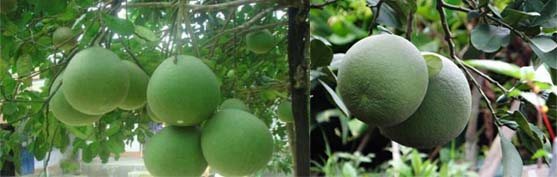
\includegraphics[width=0.8\columnwidth]{images/chap3/sample1.jpg}
    	\caption{Một vài ảnh mẫu trong tập dữ liệu đầu tiên}
    	\label{fig:my_label}
    	\end{figure}
	\end{center}
  \item Dữ liệu ảnh gồm 87 hình được chụp trực tiếp tại các vườn bưởi ở Bến Tre bằng máy ảnh kĩ thuật số. Hầu hết tất cả hình ảnh có được đều là giống bưởi da xanh và được chụp từ ngoài vào hoặc từ dưới gốc cây lên, sao cho trong ảnh vừa có cây, lá và quả. 
  	\begin{center}
    	\begin{figure}[H]
    	\centering
    	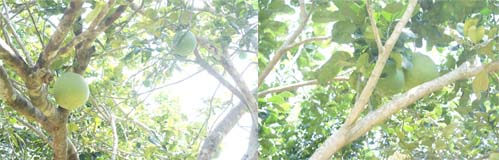
\includegraphics[width=0.7\columnwidth]{images/chap3/sample2.jpg}
    	\caption{Một vài ảnh mẫu trong tập dữ liệu thứ hai}
    	\label{fig:my_label}
    	\end{figure}
	\end{center}
Sau đó các ảnh được gán nhãn và thông qua thao tác augmentation để sinh ra tập ảnh gồm tổng cộng 10560 ảnh
\end{itemize}
\section{Tiền xử lí dữ liệu}
\subsection{Gán nhãn}
Từng trái bưởi trong các ảnh trong tập dữ liệu gốc được xác định vị trí và gán nhãn theo định dạng Pascal VOC để framework có thể đọc và thực thi (hình \ref{chap3:voc_format}).

Định dạng Pascal VOC được thể hiện dưới dạng file .xml gồm có cách trường sau:
\begin{itemize}
	\item folder
	\item filename
	\item path
	\item source
	\item size
	\begin{itemize}
		\item width
		\item height
		\item depth
	\end{itemize}
	\item segmented
	\item object
	\begin{itemize}
		\item name
		\item pose
		\item truncated 
		\item difficult
		\item bndbox
		\begin{itemize}
			\item xmin
			\item ymin
			\item xmax
			\item ymax
		\end{itemize}
	\end{itemize}
\end{itemize} 
Trong các trường trên, đối với phạm vi luận văn, ta quan tâm đến các trường size (gồm các trường width, height và depth) và object(bao gồm bndbox với các trường xmin, ymin, xmax, ymax bên trong), lần lượt là kích thước của bức ảnh đang xét và tọa độ, vị trí từng vật thể trong ảnh đó.
	\begin{center}
    	\begin{figure}[H]
    	\centering
    	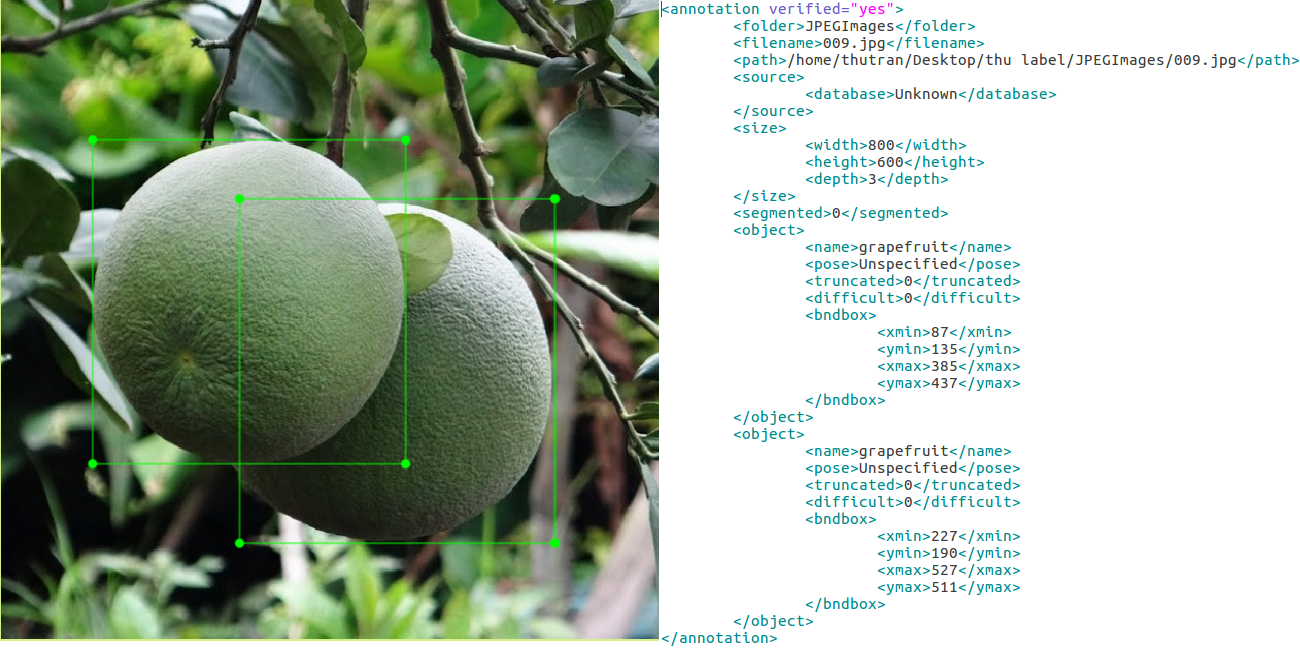
\includegraphics[width=0.7\columnwidth]{images/chap3/label.png}
    	\caption{Mỗi ảnh được mô tả bởi một file xml}
    	\label{chap3:voc_format}
    	\end{figure}
	\end{center}
Để hiện thực, ta sử dụng tool từ git sau:\\
\url{https://github.com/manhcuogntin4/Label-Annotation-VOC-Pascal} \\
Sau khi clone project về, chạy ứng dụng sẽ thấy giao diện như sau:
	\begin{center}
    	\begin{figure}[H]
    	\centering
    	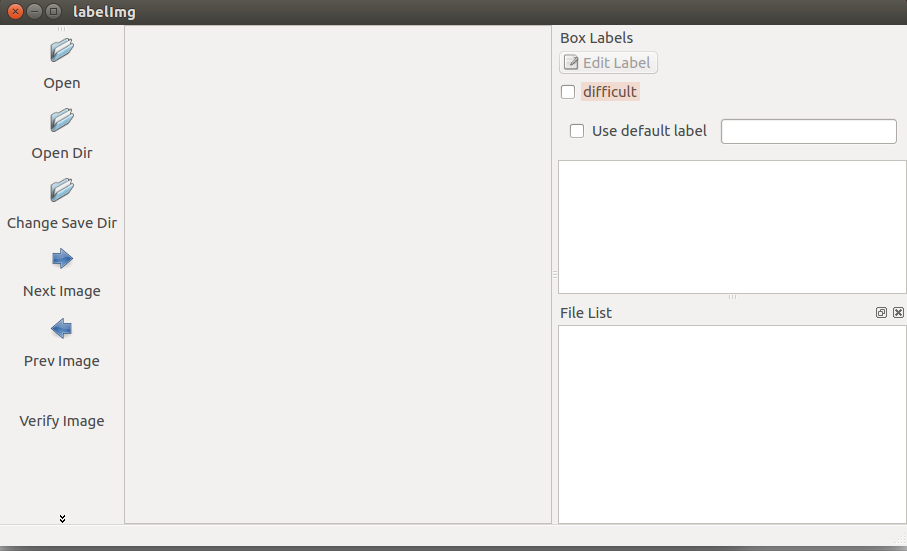
\includegraphics[width=0.7\columnwidth]{images/chap3/UI1.png}
    	\caption{Giao diên tool Pascal VOC Annotation}
    	\label{fig:my_label}
    	\end{figure}
	\end{center}
Sau khi chọn ảnh trong tập dữ liệu và label, ta có giao diện sau:
	\begin{center}
    	\begin{figure}[H]
    	\centering
    	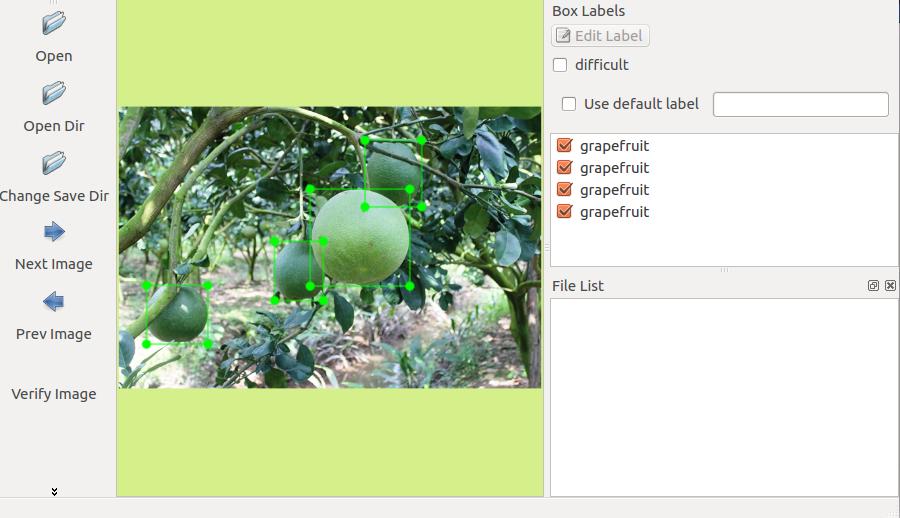
\includegraphics[width=0.7\columnwidth]{images/chap3/UI2.png}
    	\caption{Giao diên sau khi đã label}
    	\label{fig:my_label}
    	\end{figure}
	\end{center}
Để xuất file .xml, chọn Verify Image (hình \ref{chap3:verify}), file annotation sẽ được lưu cùng folder với file ảnh hoặc ở folder khác được setup trong Change Save Dir
	\begin{center}
    	\begin{figure}[H]
    	\centering
    	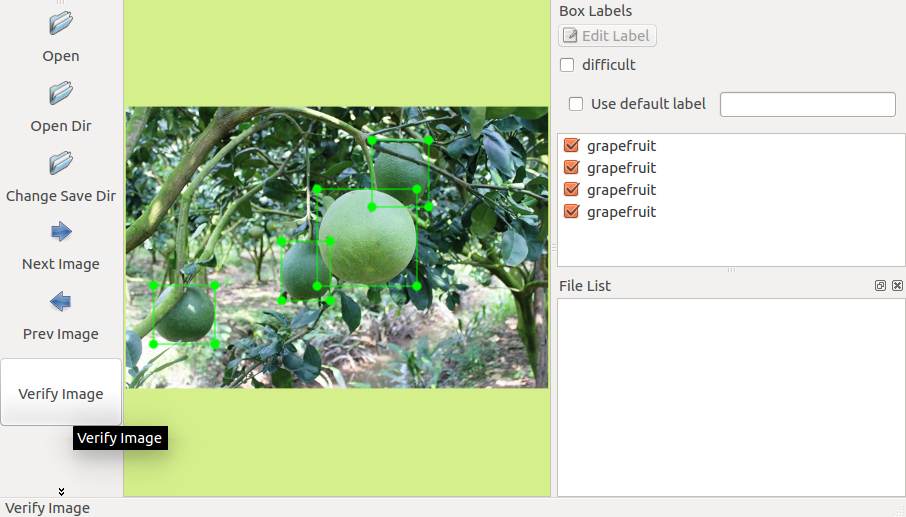
\includegraphics[width=0.7\columnwidth]{images/chap3/UI3.png}
    	\caption{Chọn Verify Image để xuất file xml}
    	\label{chap3:verify}
    	\end{figure}
	\end{center}
\cleardoublepage
Nội dung một file xml:
\begin{lstlisting}[language=XML]
<annotation verified="yes">
	<folder>JPEGImages</folder>
	<filename>001.jpg</filename>
	<path>/home/JPEGImages/001.jpg</path>
	<source>
		<database>Unknown</database>
	</source>
	<size>
		<width>640</width>
		<height>427</height>
		<depth>3</depth>
	</size>
	<segmented>0</segmented>
	<object>
		<name>grapefruit</name>
		<pose>Unspecified</pose>
		<truncated>0</truncated>
		<difficult>0</difficult>
		<bndbox>
			<xmin>290</xmin>
			<ymin>125</ymin>
			<xmax>441</xmax>
			<ymax>272</ymax>
		</bndbox>
	</object>
	<object>
		<name>grapefruit</name>
		<pose>Unspecified</pose>
		<truncated>0</truncated>
		<difficult>0</difficult>
		<bndbox>
			<xmin>42</xmin>
			<ymin>271</ymin>
			<xmax>135</xmax>
			<ymax>360</ymax>
		</bndbox>
	</object>
	<object>
		<name>grapefruit</name>
		<pose>Unspecified</pose>
		<truncated>0</truncated>
		<difficult>0</difficult>
		<bndbox>
			<xmin>373</xmin>
			<ymin>51</ymin>
			<xmax>459</xmax>
			<ymax>152</ymax>
		</bndbox>
	</object>
	<object>
		<name>grapefruit</name>
		<pose>Unspecified</pose>
		<truncated>0</truncated>
		<difficult>0</difficult>
		<bndbox>
			<xmin>236</xmin>
			<ymin>204</ymin>
			<xmax>310</xmax>
			<ymax>294</ymax>
		</bndbox>
	</object>
</annotation>
\end{lstlisting}
\subsection{Augmentation}
Data augmentation là một phương pháp rất phổ biến được dùng trong Học máy, đặc biệt là phân loại ảnh, dùng để tăng kích thước của tập dữ liệu, đồng thời tránh hiện tượng overfit.

Trong phạm vi luận văn, nhóm hiện thực các kĩ thuật cơ bản như tăng giảm độ sáng ảnh với 2 mức độ sáng và 2 mức độ tối, làm nhiễu, làm mờ, lật ảnh, xoay ảnh các góc 90, 180, 270 độ. Các thao tác augmentation được thực thi trên cả các bounding box đã được gán nhãn ở bước trước.

Sau đây là hình ảnh trước và sau khi augment của từng kĩ thuật:
	\begin{center}
    	\begin{figure}[H]
    	\centering
    	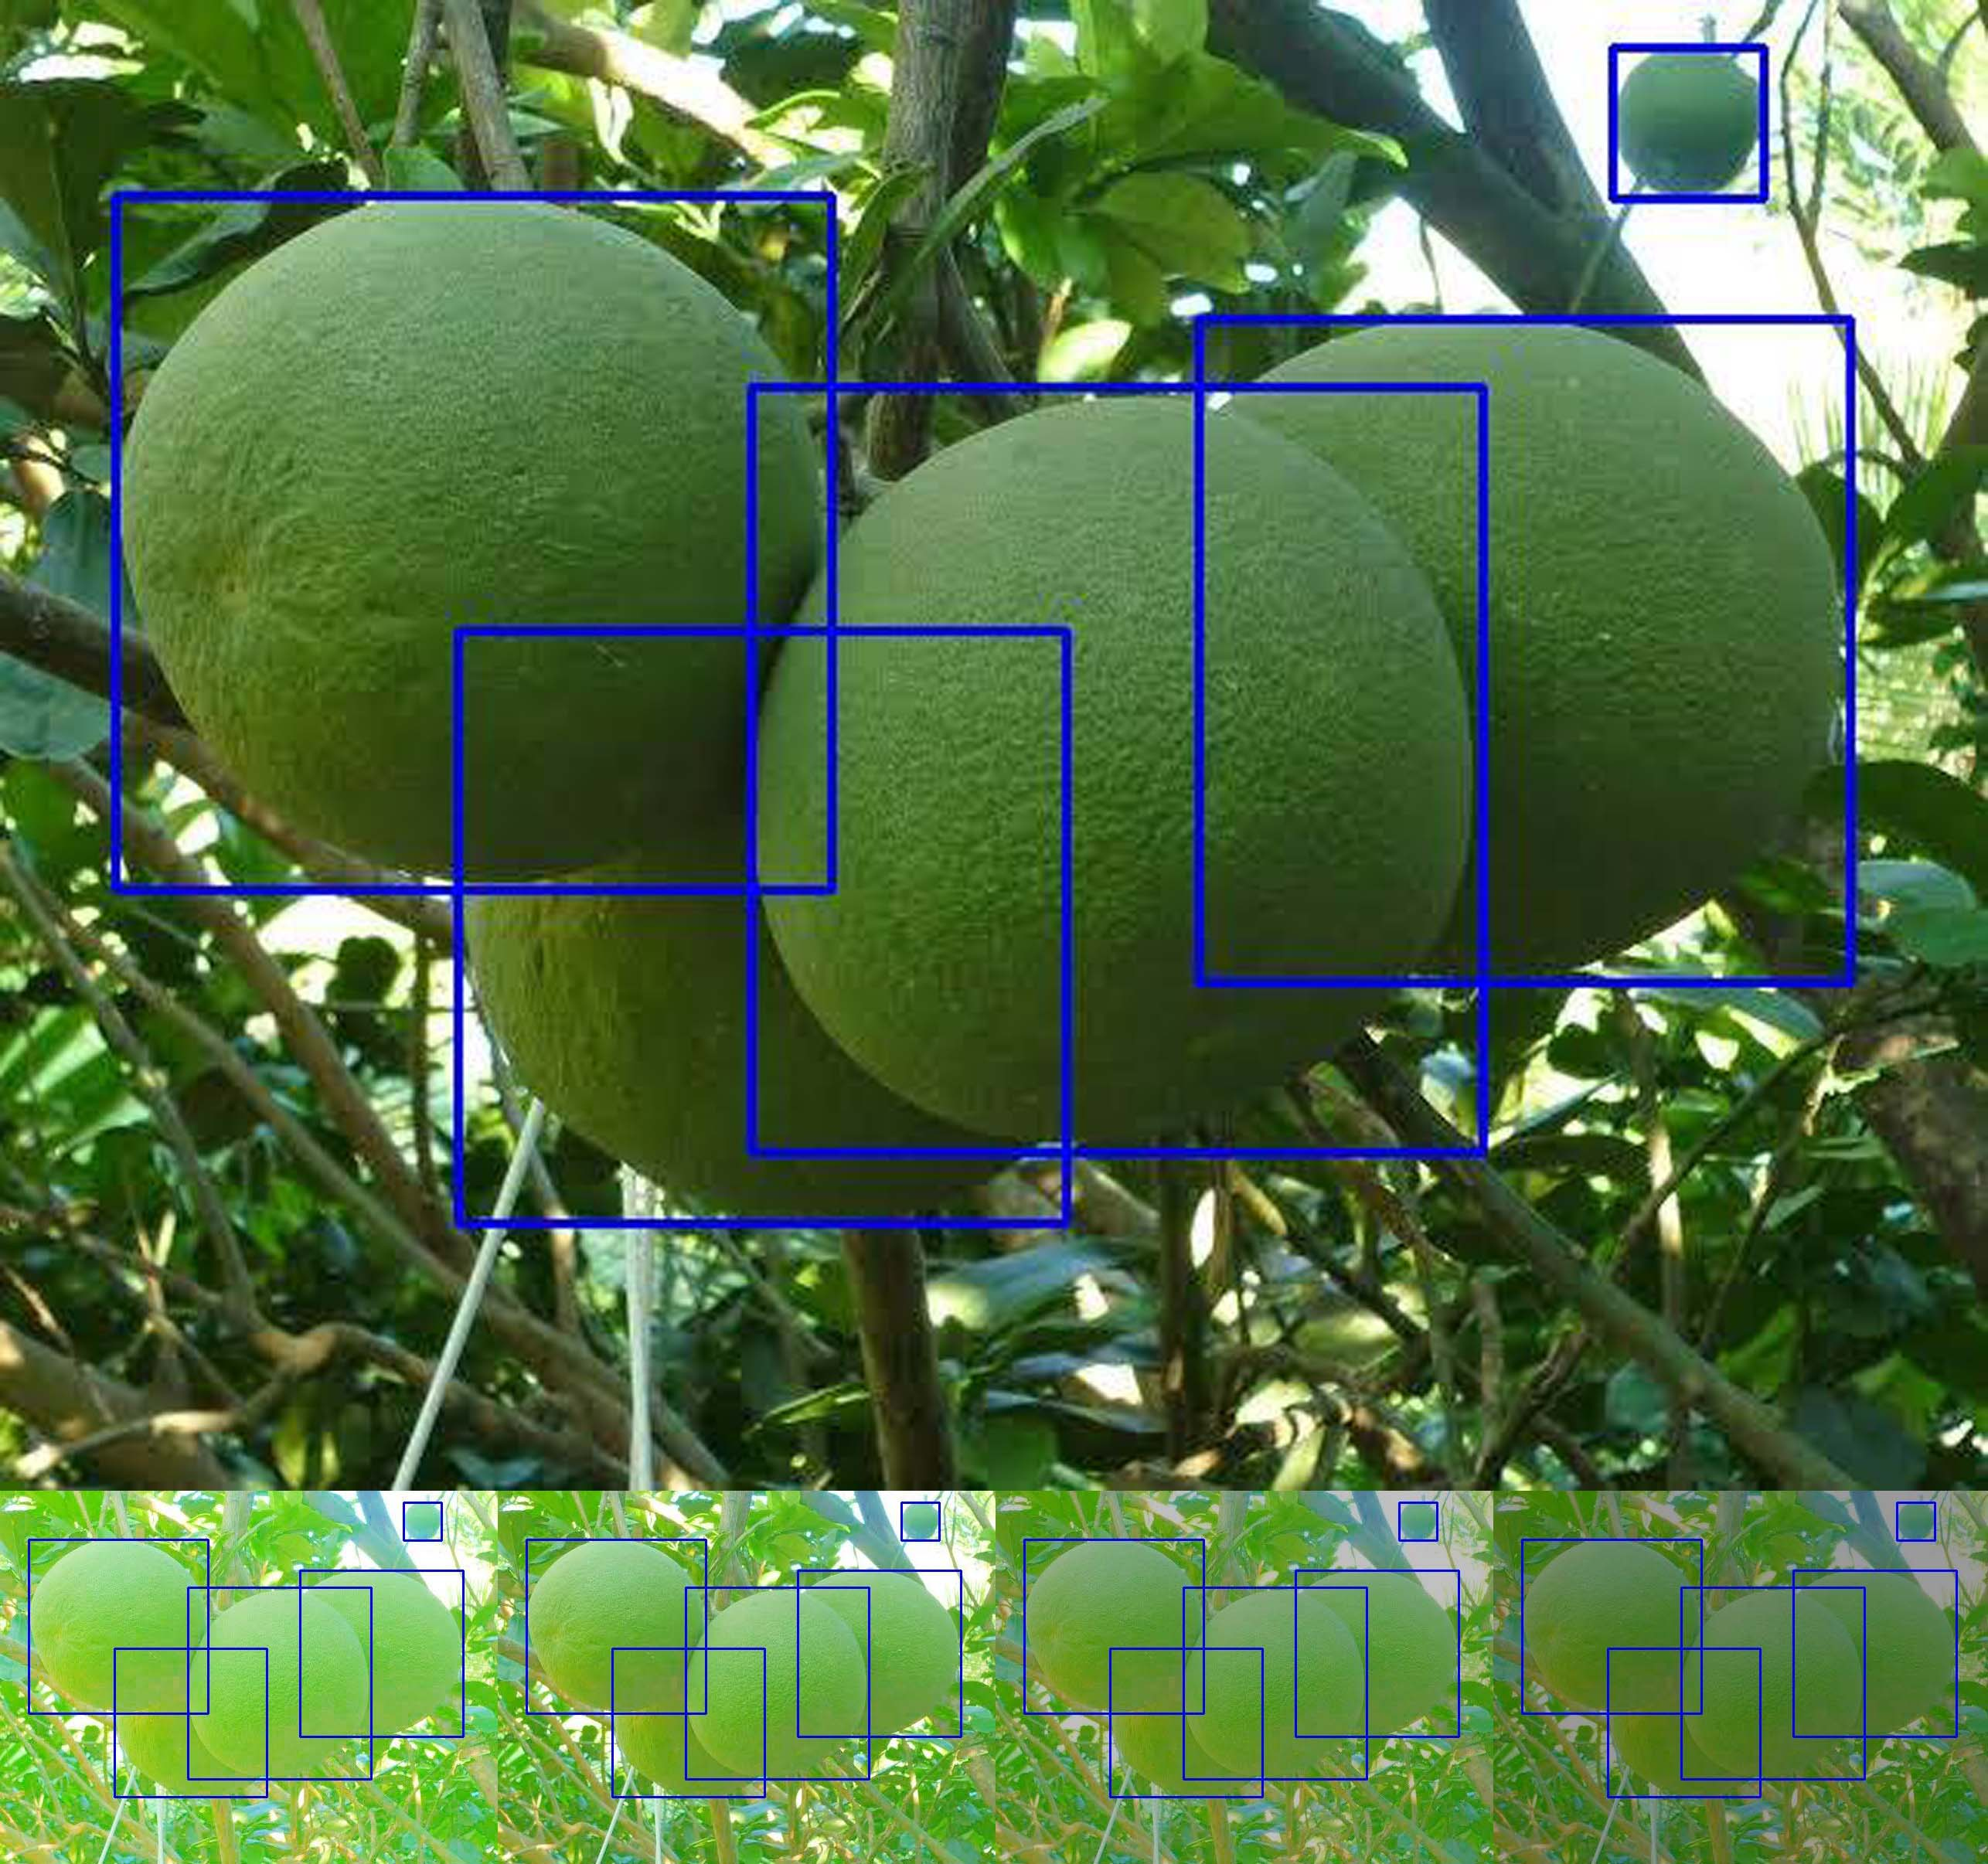
\includegraphics[width=0.6\columnwidth]{images/chap3/twerkLight.jpg}
    	\caption{Ảnh gốc đã được label và các mẫu sau khi điều chỉnh độ sáng}
    	\label{fig:my_label}
    	\end{figure}
	\end{center}
	\begin{center}
    	\begin{figure}[H]
    	\centering
    	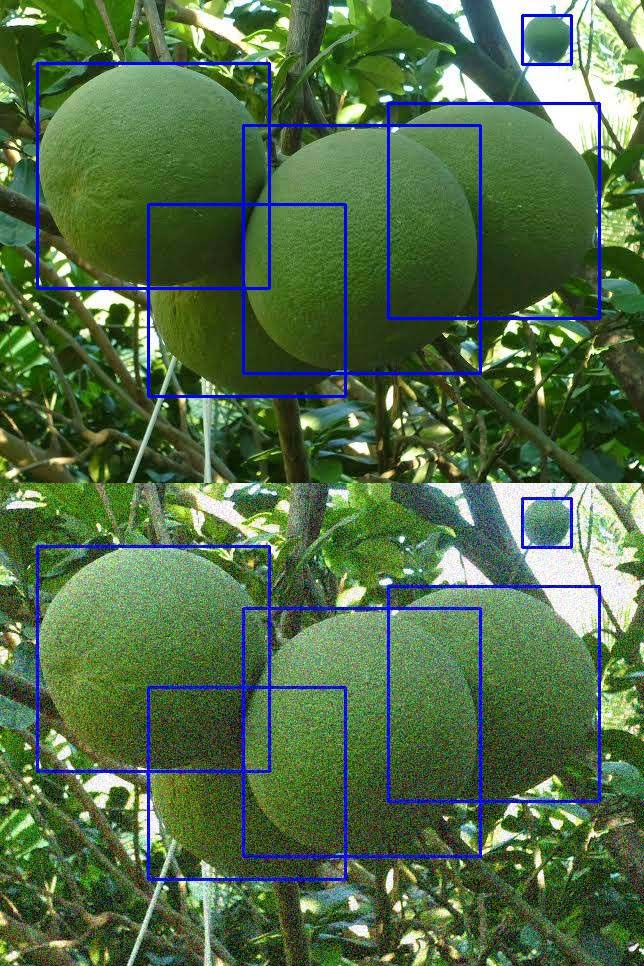
\includegraphics[width=0.4\columnwidth]{images/chap3/twerkNoise.jpg}
    	\caption{Ảnh gốc đã được label và mẫu sau khi làm nhiễu}
    	\label{fig:my_label}
    	\end{figure}
	\end{center}
	\begin{center}
    	\begin{figure}[H]
    	\centering
    	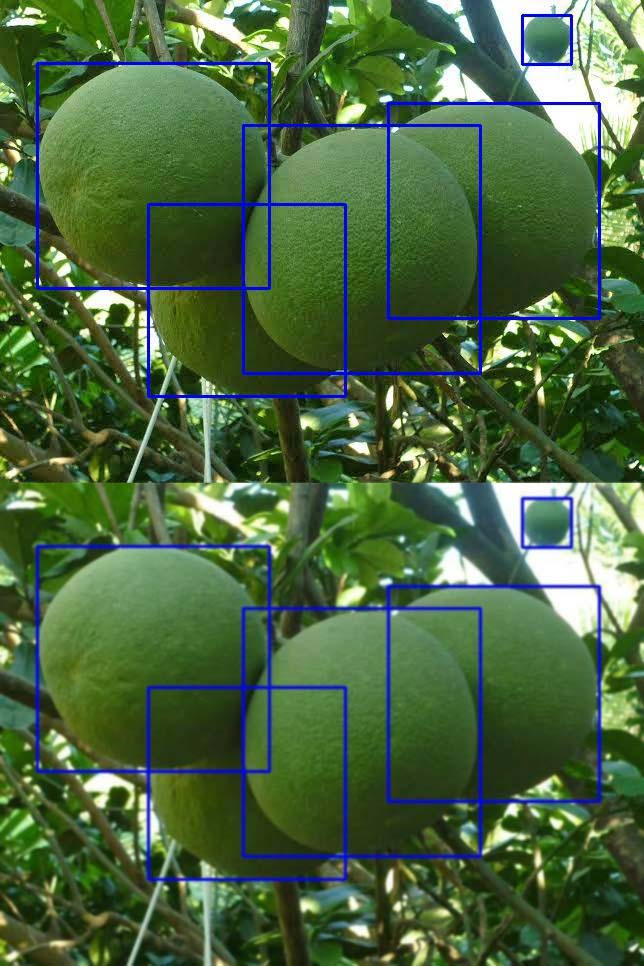
\includegraphics[width=0.4\columnwidth]{images/chap3/twerkBlur.jpg}
    	\caption{Ảnh gốc đã được label và mẫu sau khi làm mờ}
    	\label{fig:my_label}
    	\end{figure}
	\end{center}
	\begin{center}
    	\begin{figure}[H]
    	\centering
    	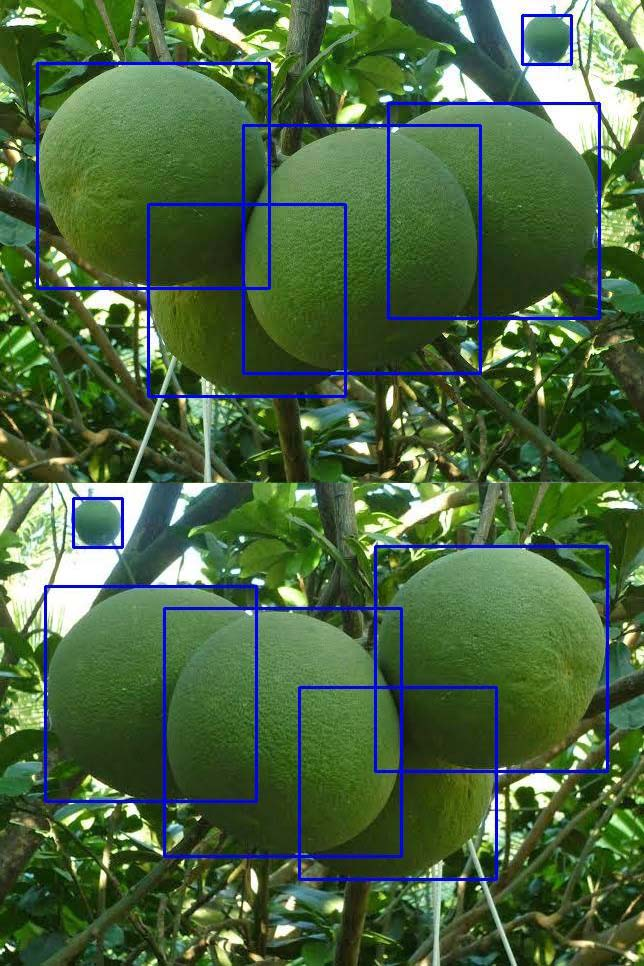
\includegraphics[width=0.4\columnwidth]{images/chap3/twerkRef.jpg}
    	\caption{Ảnh gốc đã được label và mẫu sau khi lật}
    	\label{fig:my_label}
    	\end{figure}
	\end{center}
	\begin{center}
    	\begin{figure}[H]
    	\centering
    	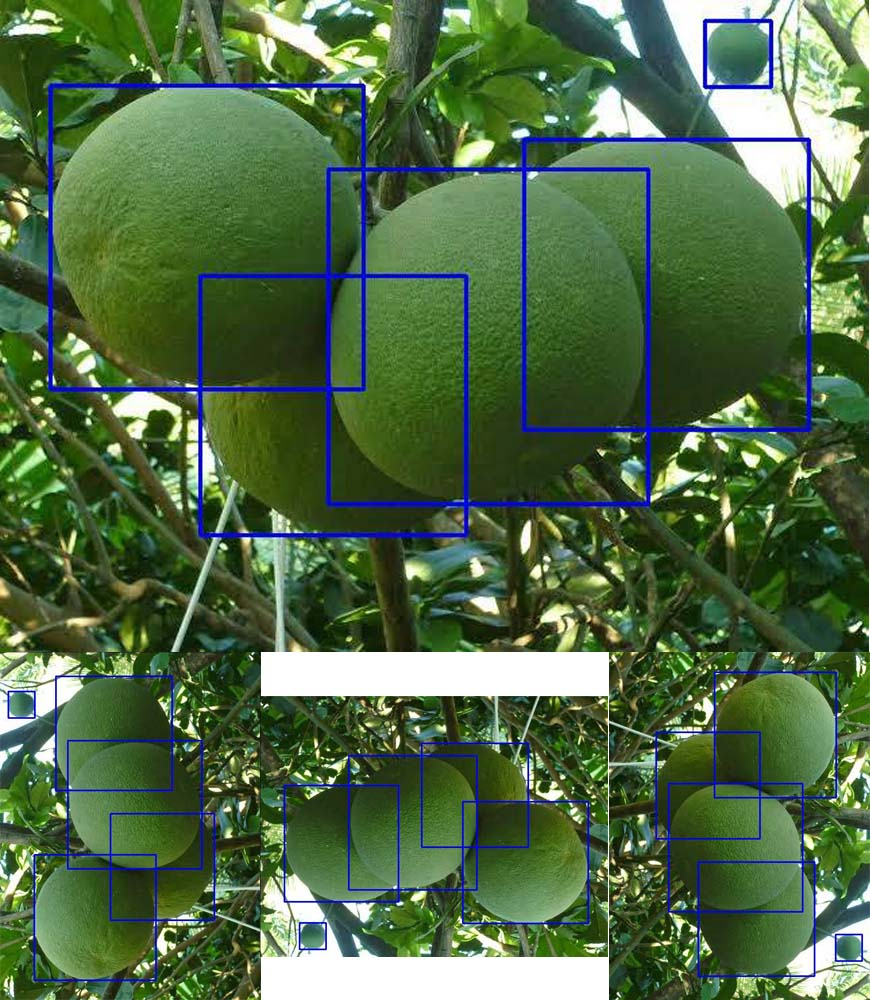
\includegraphics[width=0.4\columnwidth]{images/chap3/twerkRotate.jpg}
    	\caption{Ảnh gốc đã được label và các mẫu sau khi xoay 90, 180, 270 độ}
    	\label{fig:my_label}
    	\end{figure}
	\end{center}
Với mỗi mẫu thu được  từ một kĩ thuật augmentation, ta lại áp dụng những kĩ thuật khác lên mẫu đó. Ví dụ, ta có thể làm mờ, làm nhiễu những ảnh đã được xoay. Nhờ đó từ một ảnh ta thu được khoảng 80 ảnh, tăng kích thước tập dữ liệu.
	\begin{center}
    	\begin{figure}[H]
    	\centering
    	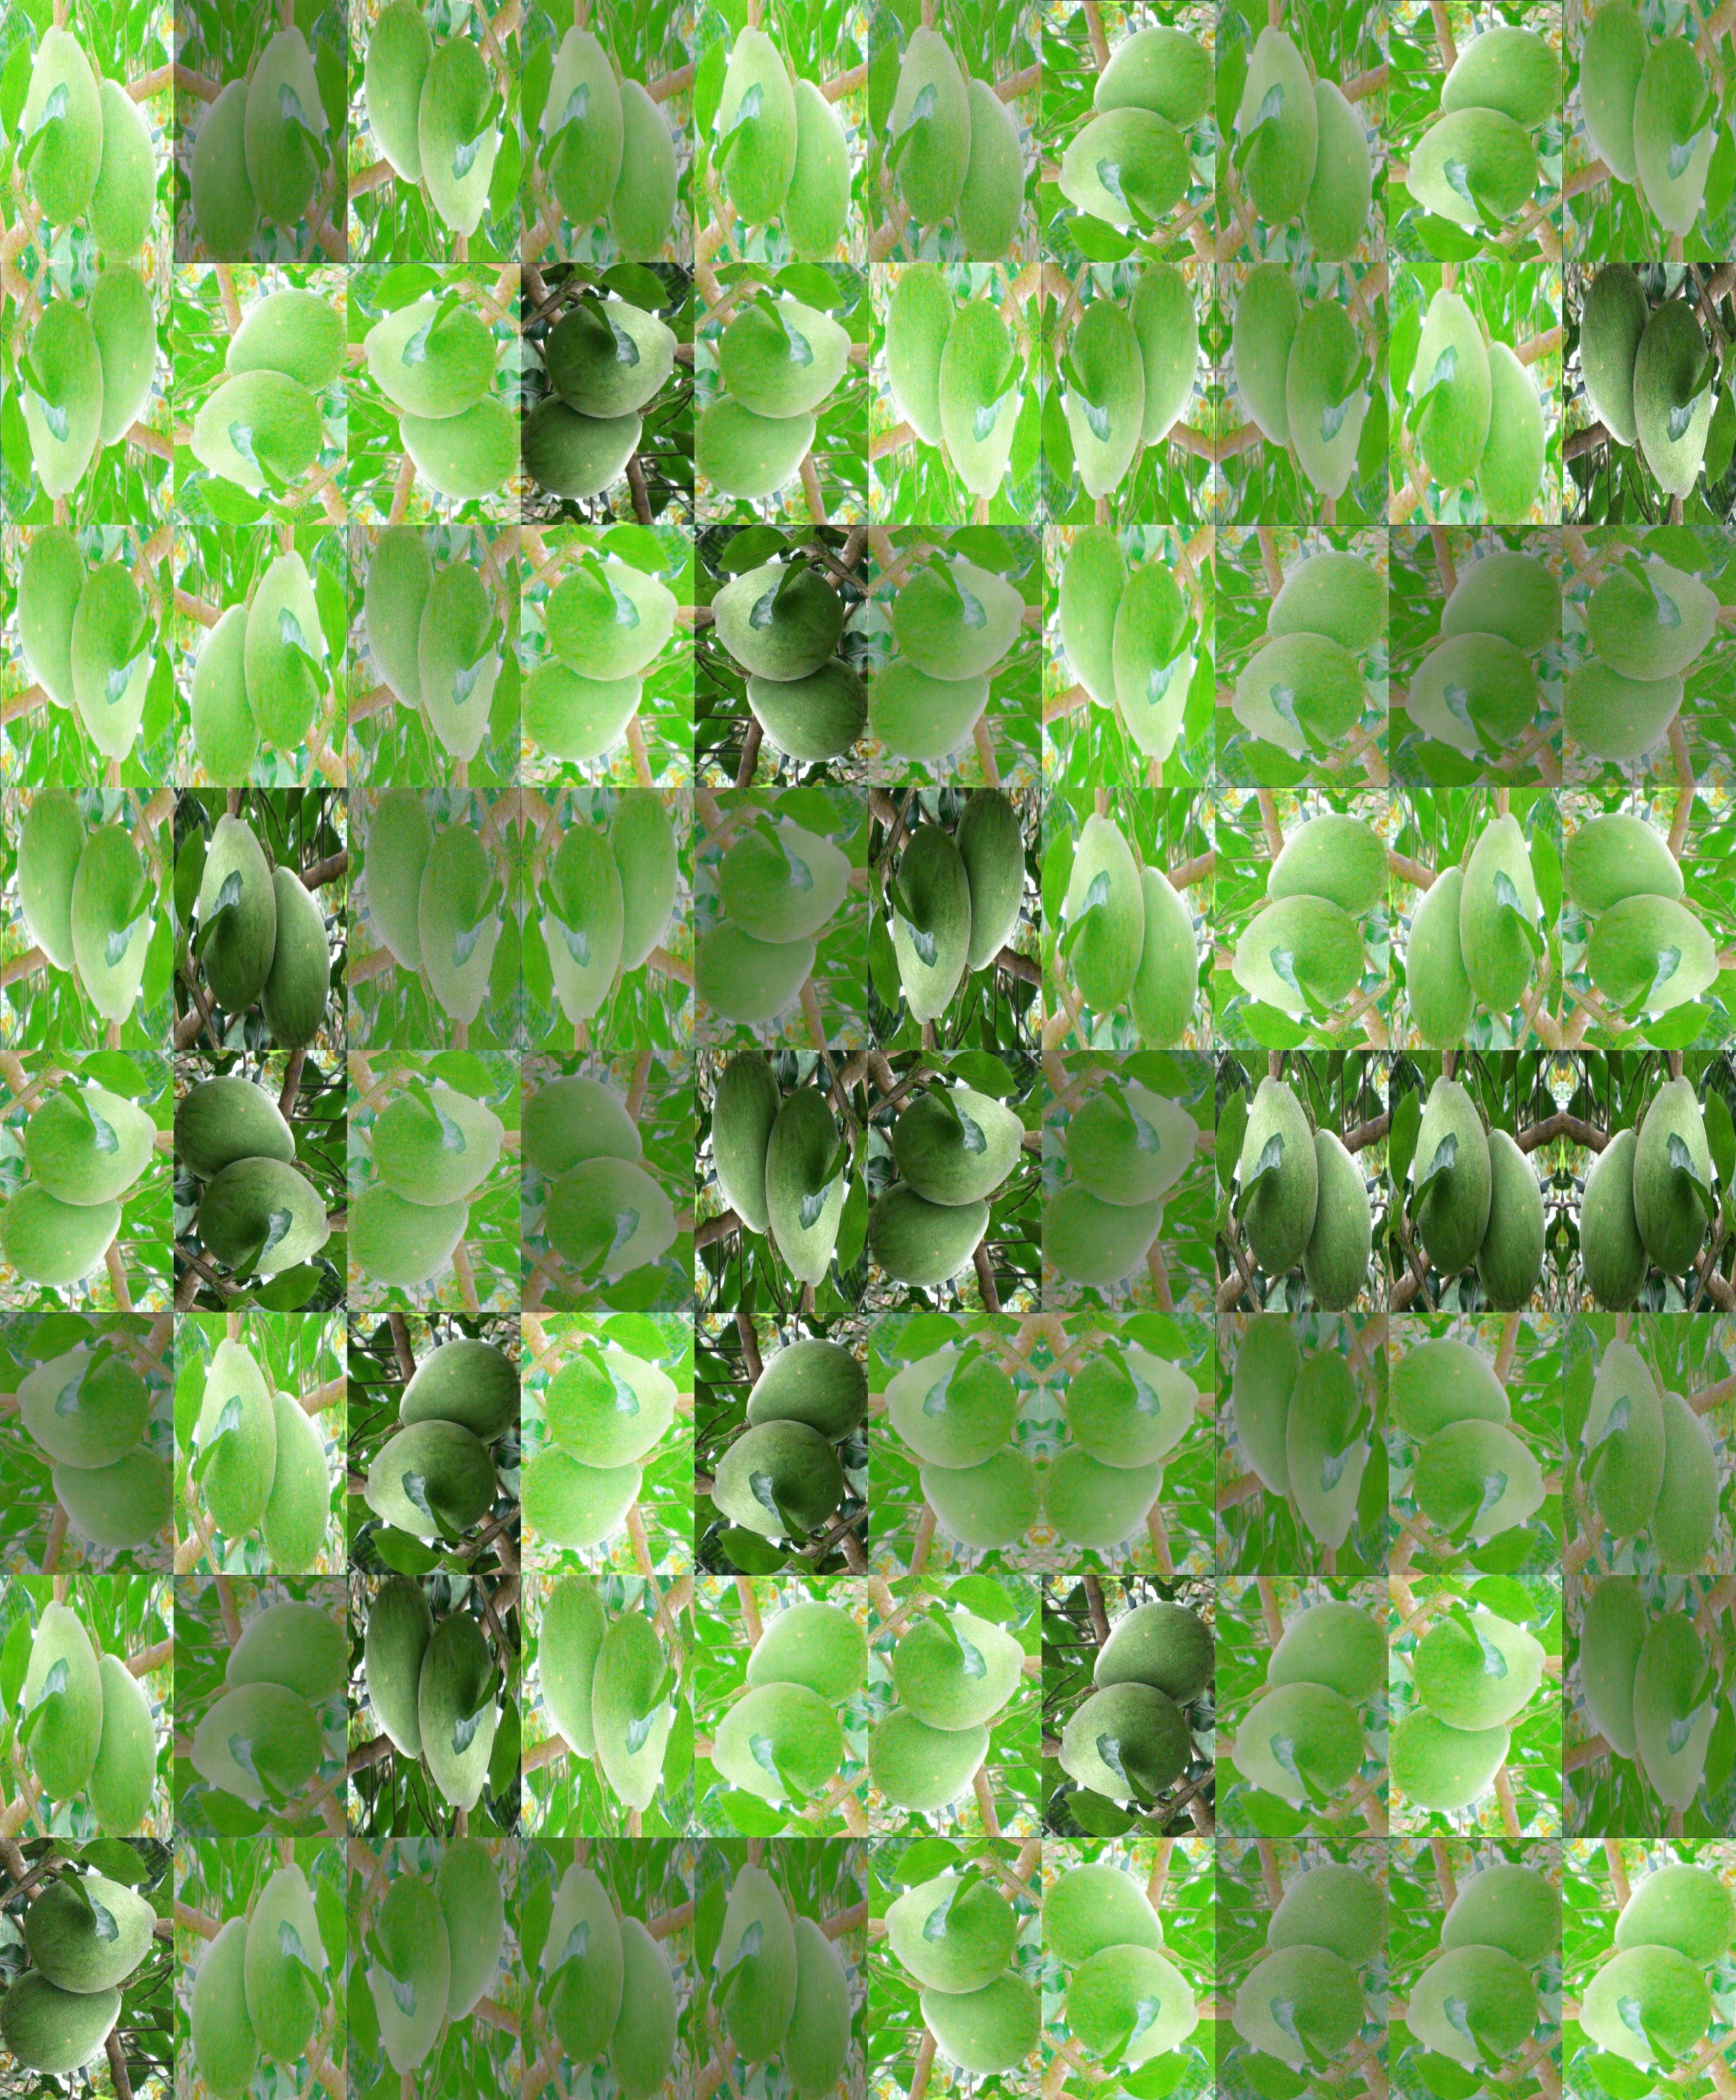
\includegraphics[width=0.4\columnwidth]{images/chap3/augment.jpg}
    	\caption{Các mẫu thu được sau khi áp dụng tất cả kĩ thuật augmentation lên một ảnh}
    	\label{fig:my_label}
    	\end{figure}
	\end{center}

\section{Quá trình huấn luyện}
\subsection{Môi trường thực hiện}
Quá trình huấn luyện thí nghiệm được thực hiện trên máy tính sử dụng vi xử lí Intel Core i3-6100, 2 nhân 4 luồng với xung nhịp 3.70 GHz, bộ nhớ RAM có dung lượng là 8 Gb, kết hợp với GPU là GTX 1080. Hệ điều hành được sử dụng là Ubuntu Desktop 18.04. 
\subsection{Mã nguồn sử dụng}
Mã nguồn mà nhóm sử dụng là mã nguồn của mô hình giải thuật Faster R-CNN được công bố trên dịch vụ mã nguồn mở Github, được viết lại bằng ngôn ngữ python kết hợp với sử dụng thư viện Tensorflow của Google, mà nguồn này được tác giả của nó mô phỏng lại từ mã nguồn chính thức sử dụng thư viện Caffe. \\ \\
Link Github mã nguồn sử dụng thư viện Tensorflow: \\
\url{https://github.com/smallcorgi/Faster-RCNN_TF} \\
\\
Link Github mã nguồn sử dụng thư viện Caffe: \\
\url{https://github.com/rbgirshick/py-faster-rcnn} \\
\subsection{Định nghĩa một số khái niệm trong huấn luyện}
\begin{itemize}
	\item Batch là lượng dữ liệu huấn luyện được truyền đi trong môt lần đẩy dự liệu vào mạng nơ-ron để huấn luyện. Đối với giải thuật Faster R-CNN, batch thường có kích thước là 1, có nghĩa là mỗi lần chỉ đưa một bức ảnh vào để huấn luyện.  
	\item Iterations là số lần dữ liệu được đẩy đi (forward) và cập nhật ngược về (backward) với số lượng mẫu huấn luyện là kích thước của batch.
	\item Mỗi epoch là mỗi lần dữ liệu được đẩy đi và cập nhật ngược về với số lượng mẫu là cả tập huấn luyện.
	\item Lấy ví dụ như có tổng cộng 256 bức ảnh trong tập dữ liệu huấn luyện, với kích thước batch là 128 bức ảnh, vậy tức là mỗi một lần huấn luyện thêm một epoch sẽ tương đương với huấn luyện thêm 2 iterations.
\end{itemize}
\cleardoublepage
\subsection{Thiết kế mô hình}
Nhóm sử dụng lại nguyên bản mô hình của gốc của giải thuật Faster R-CNN (hình \ref{chap3:original_faster}) để có thể sử dụng được transfer learning từ bộ trọng số (weights) được trích xuất sẵn của VGG, điều này giúp cho việc học các đặc trưng mới nhanh hơn rất nhiều so với việc bắt đầu học mới từ đầu.
~\\
~\\
\begin{figure}[H]
  \centering
  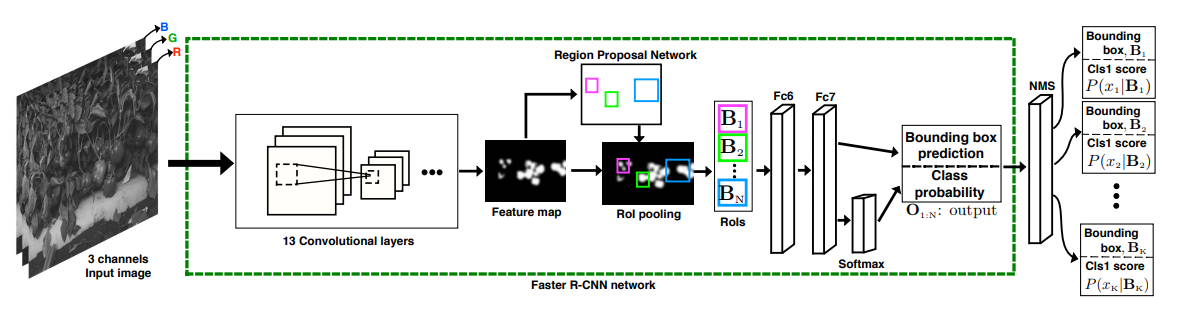
\includegraphics[width=1\textwidth]{images/chap3/fasterRCNN.png}
  \footcaption{Mô hình gốc của giải thuật Faster R-CNN}
%  \caption{Biểu đồ lỗi case 1 ở bài toán Y khoa}
  \label{chap3:original_faster}    
\end{figure}
\footnotetext{Nguồn: \cite{sa2016deepfruits}}
%\subsection{Bộ thông số}
\subsection{Chiến lược huấn luyện}
\subsubsection{Trường hợp 1}
Ở trường hợp 1, nhóm tiến hành huấn luyện mô hình với learning rate là 0.001 ở 70000 iterations đầu tiên, sau đó nhóm cho hạ learning rate và tiếp tục huấn luyện 70000 iterations nữa rồi cho dừng. 
\subsubsection{Trường hợp 2}
Ở trường hợp 2, nhóm tiến hành huấn luyện mô hình với learning rate là 0.0001.
Sau khi huấn luyện được 70000 iterations, kết quả huấn luyện cho thấy quá trình huấn luyện bắt đầu bị overfitting, được thể hiện ở việc kết quả kiểm tra có độ chính xác (Average Precision) không tăng lên mà bắt đầu giảm xuống.
\cleardoublepage
\subsection{Hàm lỗi khi huấn luyện}
\subsubsection{Trường hợp 1}
\begin{center}
    \begin{figure}[H]
    \centering
    	\begin{subfigure}[H]{0.5\linewidth}
    		\centering
    		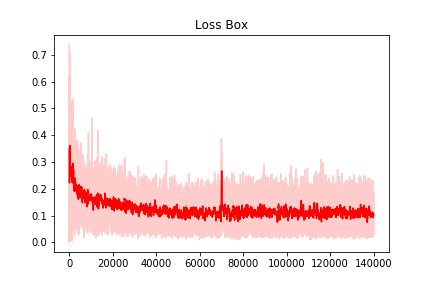
\includegraphics[width=\linewidth]{images/chap3/loss_box_2.png}
		    \caption{Biểu đồ loss box của trường hợp 1}
		    \label{fig:my_label}
		\end{subfigure}\hfill
		\begin{subfigure}[H]{0.5\linewidth}
    		\centering
    		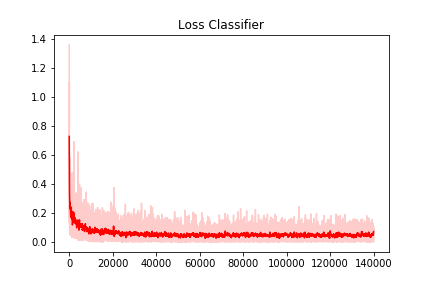
\includegraphics[width=\linewidth]{images/chap3/loss_cls_2.png}
		    \caption{Biểu đồ loss classifier của trường hợp 1}
		    \label{fig:my_label}
		\end{subfigure}\hfill
	\caption{Biểu đồ loss box và loss classifier của trường hợp 1}
    \label{fig:mylabel}
    \end{figure}

    \begin{figure}[H]
    \centering
    	\begin{subfigure}[H]{0.5\linewidth}
    		\centering
    		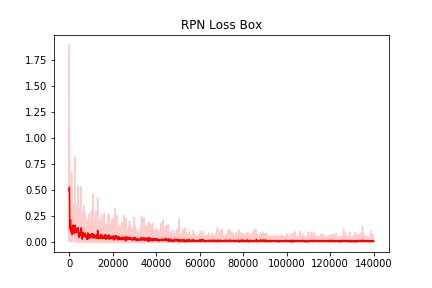
\includegraphics[width=\linewidth]{images/chap3/rpn_loss_box_2.png}
		    \caption{Biểu đồ rpn loss box của trường hợp 1}
		    \label{fig:my_label}
		\end{subfigure}\hfill
		\begin{subfigure}[H]{0.5\linewidth}
    		\centering
    		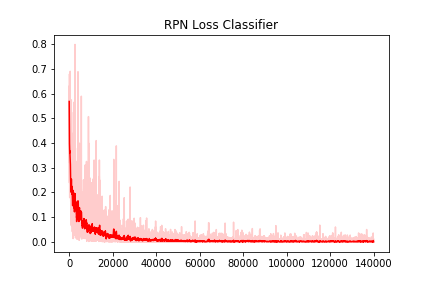
\includegraphics[width=\linewidth]{images/chap3/rpn_loss_cls_2.png}
		    \caption{Biểu đồ rpn loss classifier của trường hợp 1}
		    \label{fig:my_label}
		\end{subfigure}\hfill
	\caption{Biểu đồ rpn loss box và rpn loss classifier của trường hợp 1}
    \label{fig:mylabel}
    \end{figure}

    \begin{figure}[H]
    \centering
    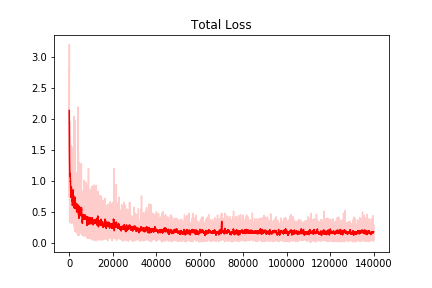
\includegraphics[width=0.9\columnwidth]{images/chap3/total_loss_2.png}
    \caption{Biểu đồ total loss của trường hợp 1}
    \label{fig:my_label}
    \end{figure}
\end{center}
\subsubsection{Trường hợp 2}
\begin{center}
	\begin{figure}[H]
    \centering
    	\begin{subfigure}[H]{0.5\linewidth}
    		\centering
    		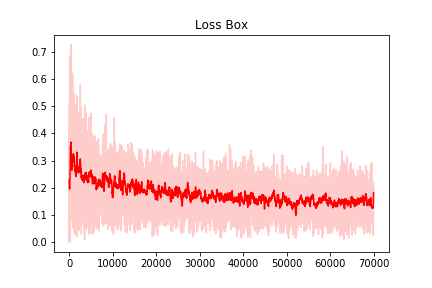
\includegraphics[width=\linewidth]{images/chap3/Loss_Box.png}
		    \caption{Biểu đồ loss box của trường hợp 2}
		    \label{fig:my_label}
		\end{subfigure}\hfill
		\begin{subfigure}[H]{0.5\linewidth}
    		\centering
    		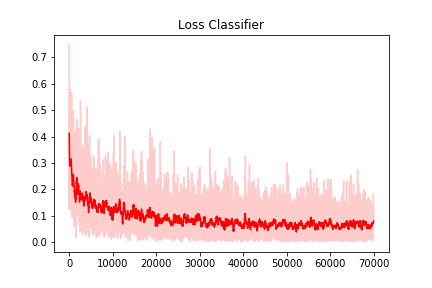
\includegraphics[width=\linewidth]{images/chap3/Loss_Classifier.png}
		    \caption{Biểu đồ loss classifier của trường hợp 2}
		    \label{fig:my_label}
		\end{subfigure}\hfill
	\caption{Biểu đồ loss box và loss classifier của trường hợp 2}
    \label{fig:mylabel}
    \end{figure}

	\begin{figure}[H]
    \centering
    	\begin{subfigure}[H]{0.5\linewidth}
    		\centering
    		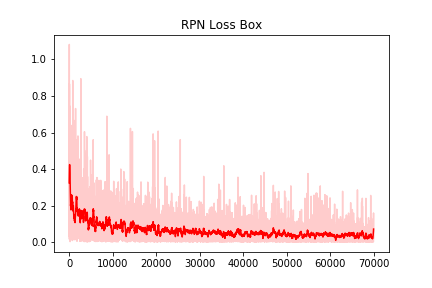
\includegraphics[width=\linewidth]{images/chap3/RPN_Loss_Box.png}
		    \caption{Biểu đồ rpn loss box của trường hợp 2}
		    \label{fig:my_label}
		\end{subfigure}\hfill
		\begin{subfigure}[H]{0.5\linewidth}
    		\centering
    		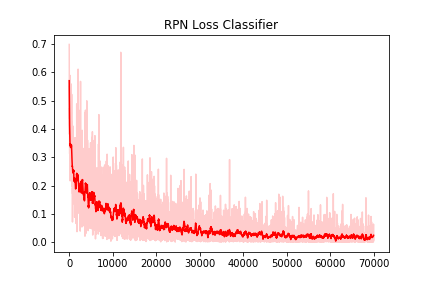
\includegraphics[width=\linewidth]{images/chap3/RPN_Loss_Classifier.png}
		    \caption{Biểu đồ rpn loss classifier của trường hợp 2}
		    \label{fig:my_label}
		\end{subfigure}\hfill
	\caption{Biểu đồ rpn loss box và rpn loss classifier của trường hợp 2}
    \label{fig:mylabel}
    \end{figure}
\end{center}

\begin{center}
    \begin{figure}[H]
    \centering
    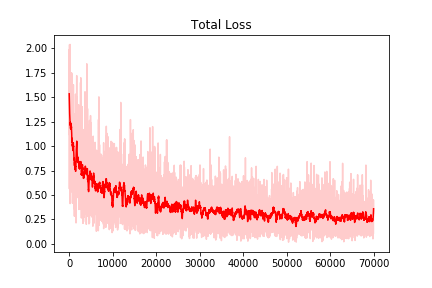
\includegraphics[width=0.9\columnwidth]{images/chap3/Total_Loss.png}
    \caption{Biểu đồ total loss của trường hợp 2}
    \label{fig:my_label}
    \end{figure}
\end{center}
\subsection{Kết quả toàn bộ tập test}
\subsubsection{Trường hợp 1}
\begin{center}
    \begin{figure}[H]
    \centering
    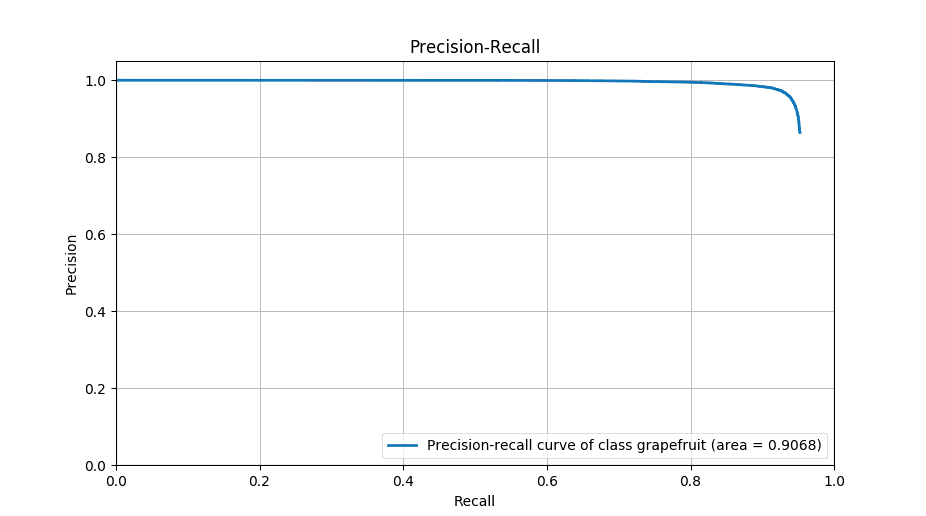
\includegraphics[width=0.9\columnwidth]{images/chap3/curve_2.png}
    \caption{Biểu đồ Precision - Recall từ kết quả kiểm tra của trường hợp 1 với toàn bộ tập test}
    \label{fig:my_label}
    \end{figure}
\end{center}
~\\
~\\
~\\
\begin{table}[H]
    \begin{tabular}{p{4cm}  p{2.5cm}  p{5.5cm} }    
    \hline		
	Tên & Giá trị & Giải thích \\
	\hline
	True Positive & 22011 & Số trái được nhận đúng \\
	False Positive & 3457  & Số trường hợp bị nhầm lẫn là trái \\
	False Negative & 1104 & Số trái mô hình chưa nhận diện được \\

    \hline
    Tổng & 23115 & Tổng số trái trong hình \\
    
    \hline
	Average Precision & 0.9068 \\
	\hline
	\end{tabular}
	\caption{Kết quả kiểm tra ở trường hợp 1 với toàn bộ tập test}
    \label{chap3:case1:table01}    
\end{table}
\begin{center}
    \begin{figure}[htp]
    \centering
    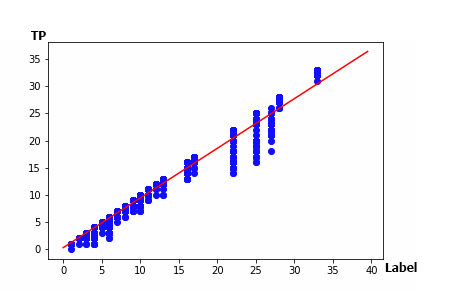
\includegraphics[width=0.9\columnwidth]{images/chap3/correlation_tp_140k.png}
    \caption{Biểu đồ tương quan từ kết quả kiểm tra của trường hợp 1 giữa TP và dữ liệu gán nhãn}
    \label{fig:my_label}
    \end{figure}
\end{center}
~\\
~\\
~\\
\begin{table}[H]
    \begin{tabular}{p{4cm}  p{2.5cm}  p{5.5cm} }
    \hline		
	Tên & Giá trị & Giải thích \\
	\hline
	\multicolumn{3}{c}{Phương trình tương quan \textbf{y = ax + b}} \\
	a & 0.91460185 & Hệ số góc \\
	b & 0.27461432 & Hệ số tự do \\
	\hline
	
	Diff & 624 & Số ảnh khác với kết quả gán nhãn \\
	Độ chính xác & 0.80303 &  Tỉ lệ số ảnh đúng trên tất cả ảnh\\
	\hline
	\end{tabular}
	\caption{Kết quả kiểm tra ở trường hợp 1 giữa TP và dữ liệu gán nhãn}
    \label{chap3:case2:table02}    
\end{table}
\subsubsection{Trường hợp 2}
\begin{center}
    \begin{figure}[H]
    \centering
    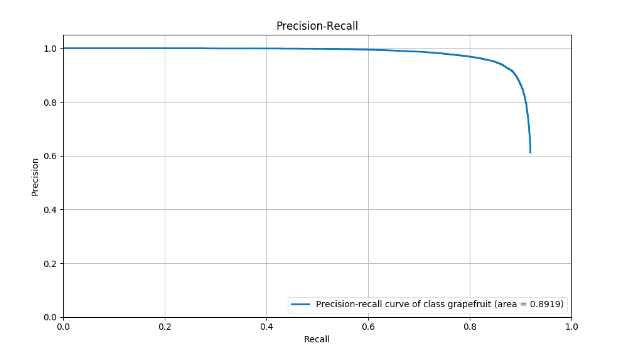
\includegraphics[width=0.9\columnwidth]{images/chap3/PR_curve.png}
    \caption{Biểu đồ Precision - Recall từ kết quả kiểm tra trường hợp 2 với toàn bộ tập test}
    \label{fig:my_label}
    \end{figure}
\end{center}
~\\
~\\
\begin{table}[H]
    \begin{tabular}{p{4cm}  p{2.5cm}  p{5.5cm} }
    \hline		
	Tên & Giá trị & Giải thích \\
	\hline
	True Positive & 21317 & Số trái được nhận đúng \\
	False Positive & 12405  & Số trường hợp bị nhầm lẫn là trái \\
	False Negative & 1798 & Số trái mô hình chưa nhận diện được \\

    \hline
    Tổng & 23115 & Tổng số trái trong hình \\
    
    \hline
	Average Precision & 0.8919\\
	\hline
	\end{tabular}
	\caption{Kết quả kiểm tra ở trường hợp 2 với toàn bộ tập test}
    \label{chap3:case2:table02}    
\end{table}
\begin{center}
    \begin{figure}[H]
    \centering
    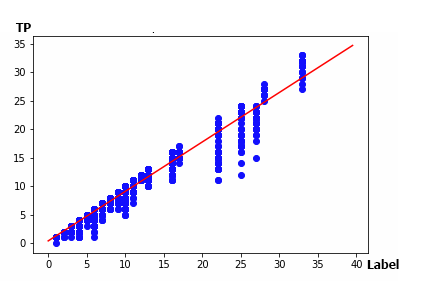
\includegraphics[width=0.9\columnwidth]{images/chap3/correlation_tp_70k.png}
    \caption{Biểu đồ tương quan của trường hợp 2 giữa TP và dữ liệu gán nhãn}
    \label{fig:my_label}
    \end{figure}
\end{center}
~\\
~\\
\begin{table}[H]
    \begin{tabular}{p{4cm}  p{2.5cm}  p{5.5cm} }   
    \hline		
	Tên & Giá trị & Giải thích \\
	\hline
	\multicolumn{3}{c}{Phương trình tương quan \textbf{y = ax + b}} \\
	a & 0.86838905 & Hệ số góc \\
	b & 0.39273578 & Hệ số tự do \\
	\hline
	Diff & 920 & Số ảnh khác với kết quả gán nhãn \\
	Độ chính xác & 0.7095959 &  Tỉ lệ số ảnh đúng trên tất cả ảnh\\
	\hline
	\end{tabular}
	\caption{Kết quả kiểm tra ở trường hợp 2 giữa TP và dữ liệu gán nhãn}
    \label{chap3:case2:table02}    
\end{table}
\subsection{Kết quả 50 mẫu trong tập test}
\subsubsection{Trường hợp 1}
\begin{center}
    \begin{figure}[H]
    \centering
    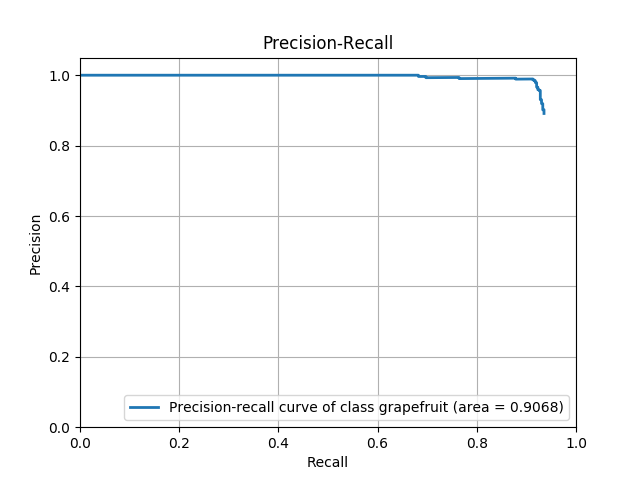
\includegraphics[width=0.9\columnwidth]{images/chap3/50_curve_140k.png}
    \caption{Biểu đồ Precision - Recall từ kết quả kiểm tra của trường hợp 1 với 50 mẫu}
    \label{fig:my_label}
    \end{figure}
\end{center}
\begin{table}[H]
    \begin{tabular}{p{4cm}  p{2.5cm}  p{5.5cm} }
    \multicolumn{3}{l}{Kết quả kiểm tra của trường hợp 1 với 50 mẫu} \\    
    \hline		
	Tên & Giá trị & Giải thích \\
	\hline
	
	True Positive & 377 & Số trái được nhận đúng\\
	False Positive & 46  & Số trường hợp bị nhầm lẫn là trái \\
	False Negative & 26 & Số trái mô hình chưa nhận diện được \\

    \hline
    Tổng & 403 & Tổng số trái trong hình \\
    
    \hline
	Average Precision & 0.9068 \\
	\hline
	\end{tabular}
	\caption{Kết quả kiểm tra ở trường hợp 1 với 50 mẫu}
    \label{chap3:case1:table01}    
\end{table}
\begin{center}
    \begin{figure}[htp]
    \centering
    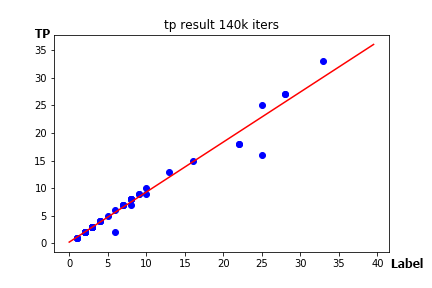
\includegraphics[width=0.9\columnwidth]{images/chap3/tp_140k.png}
    \caption{Biểu đồ tương quan từ kết quả kiểm tra của trường hợp 1 với 50 mẫu, giữa TP và dữ liệu gán nhãn}
    \label{fig:my_label}
    \end{figure}
\end{center}
~\\
~\\
\begin{table}[H]
    \begin{tabular}{p{4cm}  p{2.5cm}  p{5.5cm} }
    \hline		
	Tên & Giá trị & Giải thích \\
	\hline
	\multicolumn{3}{c}{Phương trình tương quan \textbf{y = ax + b}} \\
	a & 0.90638772 & Hệ số góc \\
	b & 0.23451492 & Hệ số tự do \\
	\hline
	Diff & 9 & Số ảnh khác với kết quả gán nhãn \\
	Độ chính xác & 0.82 &  Tỉ lệ số ảnh đúng trên tất cả ảnh\\
	\hline
	\end{tabular}
	\caption{Kết quả kiểm tra ở trường hợp 1 giữa TP và dữ liệu gán nhãn}
    \label{chap3:case2:table02}    
\end{table}
\begin{center}
    \begin{figure}[htp]
    \centering
    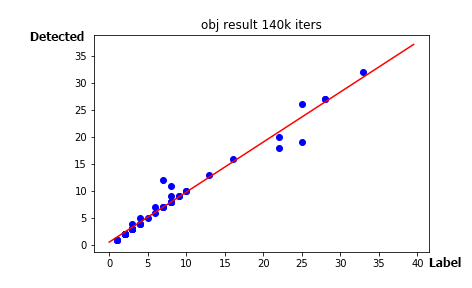
\includegraphics[width=0.9\columnwidth]{images/chap3/all_140k.png}
    \caption{Biểu đồ tương quan từ kết quả kiểm tra của trường hợp 1 với 50 mẫu , giữa các hình nhận diện được và dữ liệu gán nhãn}
    \label{fig:my_label}
    \end{figure}
\end{center}
\begin{table}[H]
    \begin{tabular}{p{4cm}  p{2.5cm}  p{5.5cm} }   
    \hline		
	Tên & Giá trị & Giải thích \\
	\hline
	\multicolumn{3}{c}{Phương trình tương quan \textbf{y = ax + b}} \\
	a & 0.92341594 & Hệ số góc \\
	b & 0.57726751 & Hệ số tự do \\
	\hline	
	Diff & 13 & Số ảnh khác với kết quả gán nhãn \\
	Độ chính xác & 0.74 &  Tỉ lệ số ảnh đúng trên tất cả ảnh\\
	\hline
	\end{tabular}
	\caption{Kết quả kiểm tra ở trường hợp 1 giữa các hình nhận diện được và dữ liệu gán nhãn}
    \label{chap3:case2:table02}    
\end{table}
\begin{table}[H]
    \begin{tabular}{p{2cm}  p{2cm}  p{2cm} p{4cm} p{2cm} }
    \hline		
	STT ảnh & TP & FP & Số object đếm được & Số label\\
	\hline
	   0   & 5  & 1  &     5     &   5   \\		\hline
   1   & 4  & 1  &     4     &   4   \\     \hline
   2   & 2  & 1  &     2     &   2   \\     \hline
   3   & 7  & 5  &     11    &   8   \\     \hline
   4   & 7  & 5  &     12    &   7   \\     \hline
   5   & 16 & 5  &     19    &   25  \\     \hline
   6   & 9  & 0  &     9     &   9   \\     \hline
   7   & 27 & 1  &     27    &   28  \\     \hline
   8   & 8  & 1  &     9     &   8   \\     \hline
   9   & 18 & 4  &     20    &   22  \\     \hline
   10  & 15 & 5  &     16    &   16  \\     \hline
   11  & 9  & 1  &     10    &   10  \\     \hline
   12  & 4  & 0  &     4     &   4   \\     \hline
   13  & 10 & 0  &     10    &   10  \\     \hline
   14  & 3  & 0  &     3     &   3   \\     \hline
   15  & 3  & 1  &     4     &   3   \\     \hline
   16  & 18 & 4  &     18    &   22  \\     \hline
   17  & 25 & 1  &     26    &   25  \\     \hline
   18  & 7  & 0  &     7     &   7   \\     \hline
   19  & 6  & 0  &     6     &   6   \\     \hline
   20  & 7  & 0  &     7     &   7   \\     \hline
   21  & 2  & 0  &     2     &   2   \\     \hline
   22  & 2  & 0  &     2     &   2   \\     \hline
   23  & 3  & 0  &     3     &   3   \\     \hline
   24  & 2  & 0  &     2     &   2   \\     \hline
   25  & 13 & 0  &     13    &   13  \\     \hline
	\end{tabular}
	\caption{Bảng số liệu đo được với 140k iters (1)}
    \label{chap3:case1:table01}    
\end{table}

\begin{table}[H]
    \begin{tabular}{p{2cm}  p{2cm}  p{2cm} p{4cm} p{2cm} }
    \hline		
	STT ảnh & TP & FP & Số object đếm được & Số label\\
	\hline
   26  & 3  & 0  &     3     &   3   \\     \hline
   27  & 1  & 0  &     1     &   1   \\     \hline
   28  & 2  & 0  &     2     &   2   \\     \hline
   29  & 7  & 1  &     7     &   7   \\     \hline
   30  & 3  & 0  &     3     &   3   \\     \hline
   31  & 3  & 0  &     3     &   3   \\     \hline
   32  & 27 & 0  &     27    &   28  \\     \hline
   33  & 8  & 0  &     8     &   8   \\     \hline
   34  & 2  & 0  &     2     &   2   \\     \hline
   35  & 2  & 0  &     2     &   2   \\     \hline
   36  & 8  & 0  &     8     &   8   \\     \hline
   37  & 4  & 1  &     5     &   4   \\     \hline
   38  & 9  & 1  &     9     &   9   \\     \hline
   39  & 2  & 5  &     7     &   6   \\     \hline
   40  & 4  & 0  &     4     &   4   \\     \hline
   41  & 3  & 2  &     3     &   3   \\     \hline
   42  & 8  & 0  &     8     &   8   \\     \hline
   43  & 1  & 0  &     1     &   1   \\     \hline
   44  & 3  & 0  &     3     &   3   \\     \hline
   45  & 1  & 0  &     1     &   1   \\     \hline
   46  & 8  & 0  &     8     &   8   \\     \hline
   47  & 2  & 0  &     2     &   2   \\     \hline
   48  & 1  & 0  &     1     &   1   \\     \hline
   49  & 33 & 0  &     32    &   33  \\     \hline


	\end{tabular}
	\caption{Bảng số liệu đo được với 140k iters (2)}
    \label{chap3:case1:table01}    
\end{table}

\subsubsection{Trường hợp 2}
\begin{center}
    \begin{figure}[H]
    \centering
    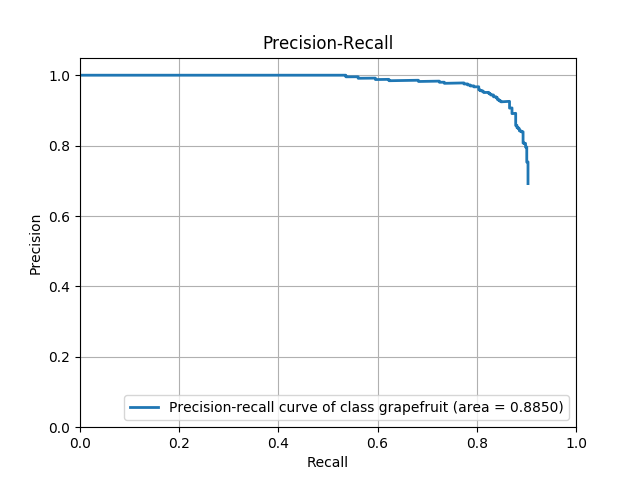
\includegraphics[width=0.9\columnwidth]{images/chap3/50_curve_70k.png}
    \caption{Biểu đồ Precision - Recall từ kết quả kiểm tra trường hợp 2 với 50 mẫu}
    \label{fig:my_label}
    \end{figure}
\end{center}
\begin{table}[H]
    \begin{tabular}{p{4cm}  p{2.5cm}  p{5.5cm} }
    \multicolumn{3}{l}{Kết quả kiểm tra của trường hợp 2 với 50 mẫu} \\    
    \hline		
	Tên & Giá trị & Giải thích \\
	\hline
	True Positive & 364 & Số trái được nhận đúng \\
	False Positive & 162  & Số trường hợp bị nhầm lẫn là trái \\
	False Negative & 39 & Số trái mô hình chưa nhận diện được \\
    \hline
    Tổng & 403 & Tổng số trái trong hình \\
    \hline
	Average Precision & 0.8850\\
	\hline
	\end{tabular}
	\caption{Kết quả kiểm tra ở trường hợp 2 với 50 mẫu}
    \label{chap3:case2:table02}    
\end{table}
\begin{center}
    \begin{figure}[H]
    \centering
    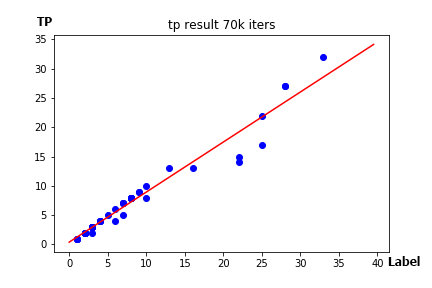
\includegraphics[width=0.9\columnwidth]{images/chap3/tp_70k.png}
    \caption{Biểu đồ tương quan của trường hợp 2 với 50 mẫu, giữa TP và dữ liệu gán nhãn}
    \label{fig:my_label}
    \end{figure}
\end{center}
\begin{table}[H]
    \begin{tabular}{p{4cm}  p{2.5cm}  p{5.5cm} }   
    \hline		
	Tên & Giá trị & Giải thích \\
	\hline
	\multicolumn{3}{c}{Phương trình tương quan \textbf{y = ax + b}} \\
	a & 0.85391164 & Hệ số góc \\
	b & 0.39747212 & Hệ số tự do \\
	\hline	
	Diff & 12 & Số ảnh khác với kết quả gán nhãn \\
	Độ chính xác & 0.76 &  Tỉ lệ số ảnh đúng trên tất cả ảnh\\
	\hline
	\end{tabular}
	\caption{Kết quả kiểm tra ở trường hợp 2 giữa TP và dữ liệu gán nhãn}
    \label{chap3:case2:table02}    
\end{table}
\begin{center}
    \begin{figure}[H]
    \centering
    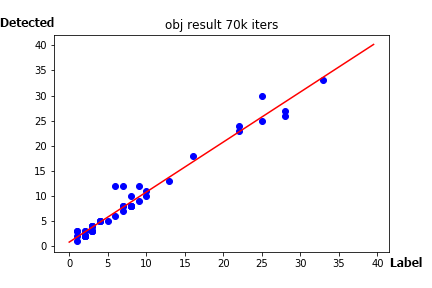
\includegraphics[width=0.9\columnwidth]{images/chap3/all_70k.png}
    \caption{Biểu đồ tương quan của trường hợp 2 với 50 mẫu, giữa các hình nhận diện được và dữ liệu gán nhãn}
    \label{fig:my_label}
    \end{figure}
\end{center}
\begin{table}[H]
    \begin{tabular}{p{4cm}  p{2.5cm}  p{5.5cm} }   
    \hline		
	Tên & Giá trị & Giải thích \\
	\hline
	\multicolumn{3}{c}{Phương trình tương quan \textbf{y = ax + b}} \\
	a & 0.99495528 & Hệ số góc \\
	b & 0.86066041 & Hệ số tự do \\
	\hline
	Diff & 12 & Số ảnh khác với kết quả gán nhãn \\
	Độ chính xác & 0.48 &  Tỉ lệ số ảnh đúng trên tất cả ảnh\\
	\hline
	\end{tabular}
	\caption{Kết quả kiểm tra ở trường hợp 2 giữa các hình nhận diện được và dữ liệu gán nhãn}
    \label{chap3:case2:table02}    
\end{table}
\begin{table}[H]
    \begin{tabular}{p{2cm}  p{2cm}  p{2cm} p{4cm} p{2cm} }
    \hline		
	STT ảnh & TP & FP & Số object đếm được & Số label\\
	\hline
	0   & 5  & 1  &     5     &   5   \\		
	\hline
	1   & 4  & 3  &     5     &   4   \\     
	\hline
	2   & 2  & 2  &     2     &   2   \\     
	\hline
	3   & 8  & 7  &     10    &   8   \\     
	\hline
	4   & 5  & 13 &     12    &   7   \\     
	\hline
	5   & 17 & 24 &     30    &   25  \\     
	\hline
	6   & 9  & 0  &     9     &   9   \\     
	\hline
	7   & 27 & 0  &     27    &   28  \\     
	\hline
	8   & 8  & 0  &     8     &   8   \\     
	\hline
	9   & 14 & 17 &     24    &   22  \\     
	\hline
	10  & 13 & 15 &     18    &   16  \\     
	\hline
	11  & 10 & 5  &     11    &   10  \\     
	\hline
	12  & 4  & 1  &     5     &   4   \\     
	\hline
	13  & 8  & 2  &     10    &   10  \\     
	\hline
	14  & 3  & 0  &     3     &   3   \\     
	\hline
	15  & 3  & 2  &     4     &   3   \\     
	\hline
	16  & 15 & 18 &     23    &   22  \\     
	\hline
	17  & 22 & 7  &     25    &   25  \\     
	\hline
	18  & 7  & 1  &     8     &   7   \\     
	\hline
	19  & 6  & 0  &     6     &   6   \\     
	\hline
	20  & 7  & 2  &     8     &   7   \\     
	\hline
	21  & 2  & 1  &     3     &   2   \\     
	\hline
	22  & 2  & 0  &     2     &   2   \\     
	\hline
	23  & 2  & 2  &     4     &   3   \\     
	\hline
	24  & 2  & 1  &     3     &   2   \\     
	\hline
	25  & 13 & 1  &     13    &   13  \\     
	\end{tabular}
	\caption{Bảng số liệu đo được với 70k iters (1)}
    \label{chap3:case1:table01}    
\end{table}

\begin{table}[H]
    \begin{tabular}{p{2cm}  p{2cm}  p{2cm} p{4cm} p{2cm} }
    \hline		
	STT ảnh & TP & FP & Số object đếm được & Số label\\
	\hline
	26  & 3  & 0  &     3     &   3   \\     
	\hline
	27  & 1  & 3  &     3     &   1   \\     
	\hline
	28  & 2  & 0  &     2     &   2   \\     
	\hline
	29  & 7  & 0  &     7     &   7   \\     
	\hline
	30  & 3  & 0  &     3     &   3   \\     
	\hline
	31  & 3  & 0  &     3     &   3   \\     
	\hline
	32  & 27 & 0  &     26    &   28  \\     
	\hline
	33  & 8  & 1  &     8     &   8   \\     
	\hline
	34  & 2  & 1  &     2     &   2   \\     
	\hline
	35  & 2  & 1  &     2     &   2   \\     
	\hline
	36  & 8  & 0  &     8     &   8   \\     
	\hline
	37  & 4  & 1  &     5     &   4   \\     
	\hline
	38  & 9  & 5  &     12    &   9   \\     
	\hline
	39  & 4  & 10 &     12    &   6   \\     
	\hline
	40  & 4  & 1  &     5     &   4   \\     
	\hline
	41  & 3  & 3  &     4     &   3   \\     
	\hline
	42  & 8  & 0  &     8     &   8   \\     
	\hline
	43  & 1  & 2  &     2     &   1   \\     
	\hline
	44  & 3  & 3  &     4     &   3   \\     
	\hline
	45  & 1  & 0  &     1     &   1   \\     
	\hline
	46  & 8  & 1  &     8     &   8   \\     
	\hline
	47  & 2  & 1  &     2     &   2   \\     
	\hline
	48  & 1  & 2  &     3     &   1   \\     
	\hline
	49  & 32 & 2  &     33    &   33  \\     
	\hline

	\end{tabular}
	\caption{Bảng số liệu đo được với 70k iters (2)}
    \label{chap3:case1:table01}    
\end{table}
\subsection{Demo}
Hình \ref{chap3:good} cho kết quả rất tốt, nhận diện đủ số lượng đối với trường hợp vật thể có mặt trong ảnh rõ ràng và ít bị khuất.
\begin{center}
    \begin{figure}[H]
    \centering
    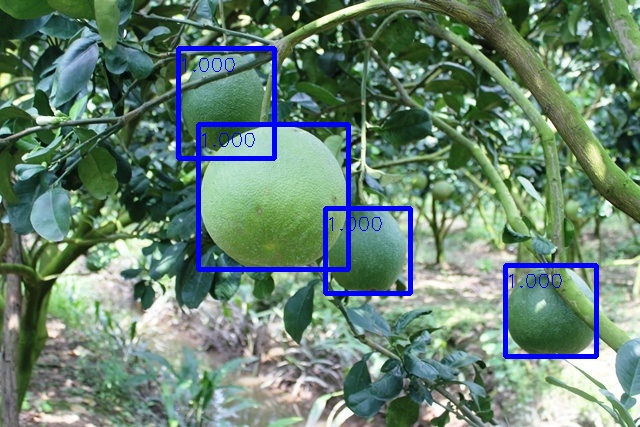
\includegraphics[width=0.6\columnwidth]{images/chap3/demo_001.jpg}
    \caption{Một số hình ảnh demo}
    \label{chap3:good}
    \end{figure}
\end{center}

Hình \ref{chap3:good1}, \ref{chap3:good2} cũng cho kết quả khá tốt trong trường hợp số lượng trái nhiều, rõ và bị khuất bởi lá ít. 
\begin{center}
    \begin{figure}[H]
    \centering
    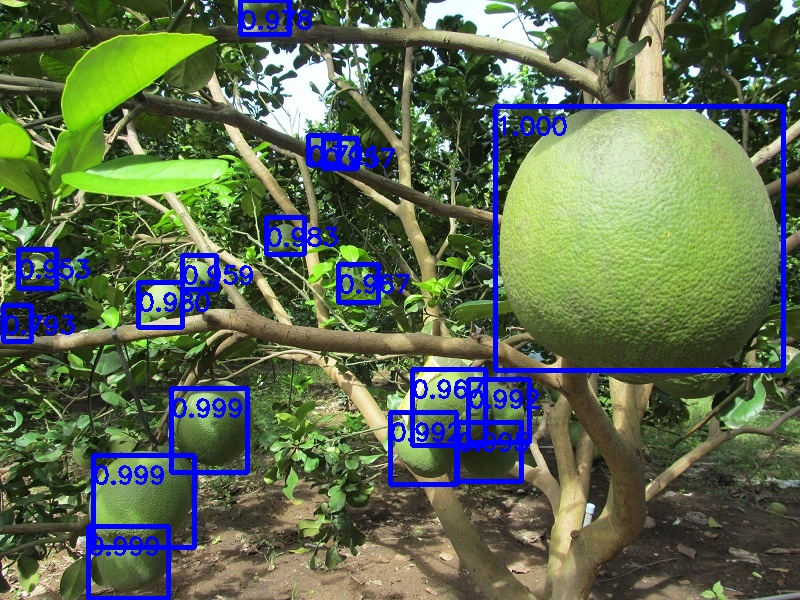
\includegraphics[width=0.6\columnwidth]{images/chap3/demo_002.jpg}
    \caption{Một số hình ảnh demo}
    \label{chap3:good1}
    \end{figure}
\end{center}

\begin{center}
    \begin{figure}[H]
    \centering
    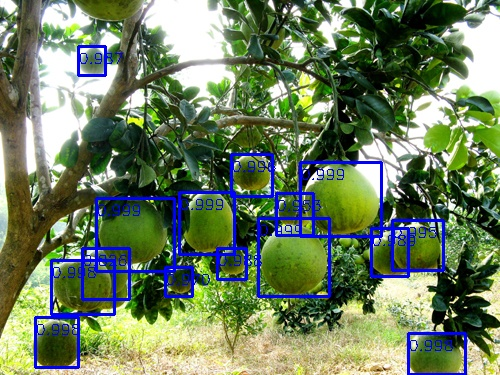
\includegraphics[width=0.6\columnwidth]{images/chap3/demo_004.jpg}
    \caption{Một số hình ảnh demo}
    \label{chap3:good2}
    \end{figure}
\end{center}
Đối với các hình bị làm mờ, nhiễu, và thay đổi độ sáng với các trái ở gần rõ và ít bị che, kết quả nhận diện vẫn tốt.
\begin{center}
    \begin{figure}[H]
    \centering
    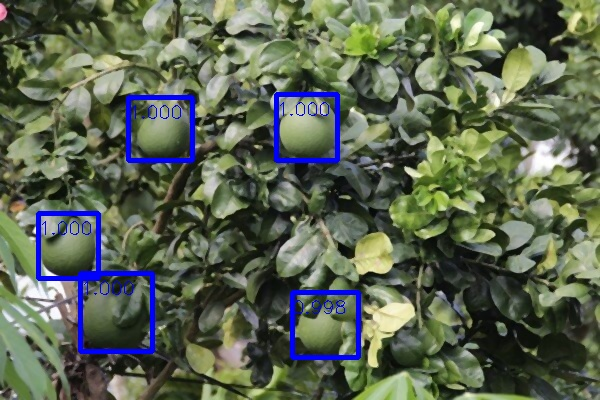
\includegraphics[width=0.6\columnwidth]{images/chap3/demo_006.jpg}
    \caption{Kết quả nhận diện với hình ảnh bị làm mờ}
    \label{chap3:good4}
    \end{figure}
\end{center}
\begin{center}
    \begin{figure}[H]
    \centering
    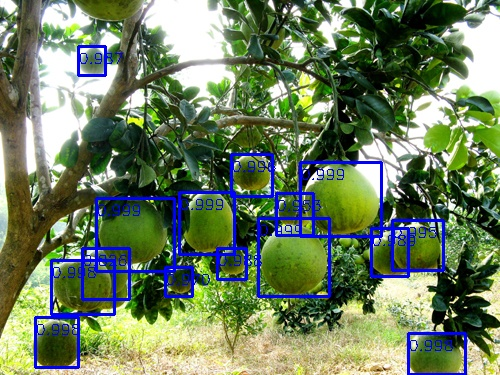
\includegraphics[width=0.6\columnwidth]{images/chap3/demo_007.jpg}
    \caption{Kết quả nhận diện với hình ảnh bị nhiễu}
    \label{chap3:good5}
    \end{figure}
\end{center}

\begin{center}
    \begin{figure}[H]
    \centering
    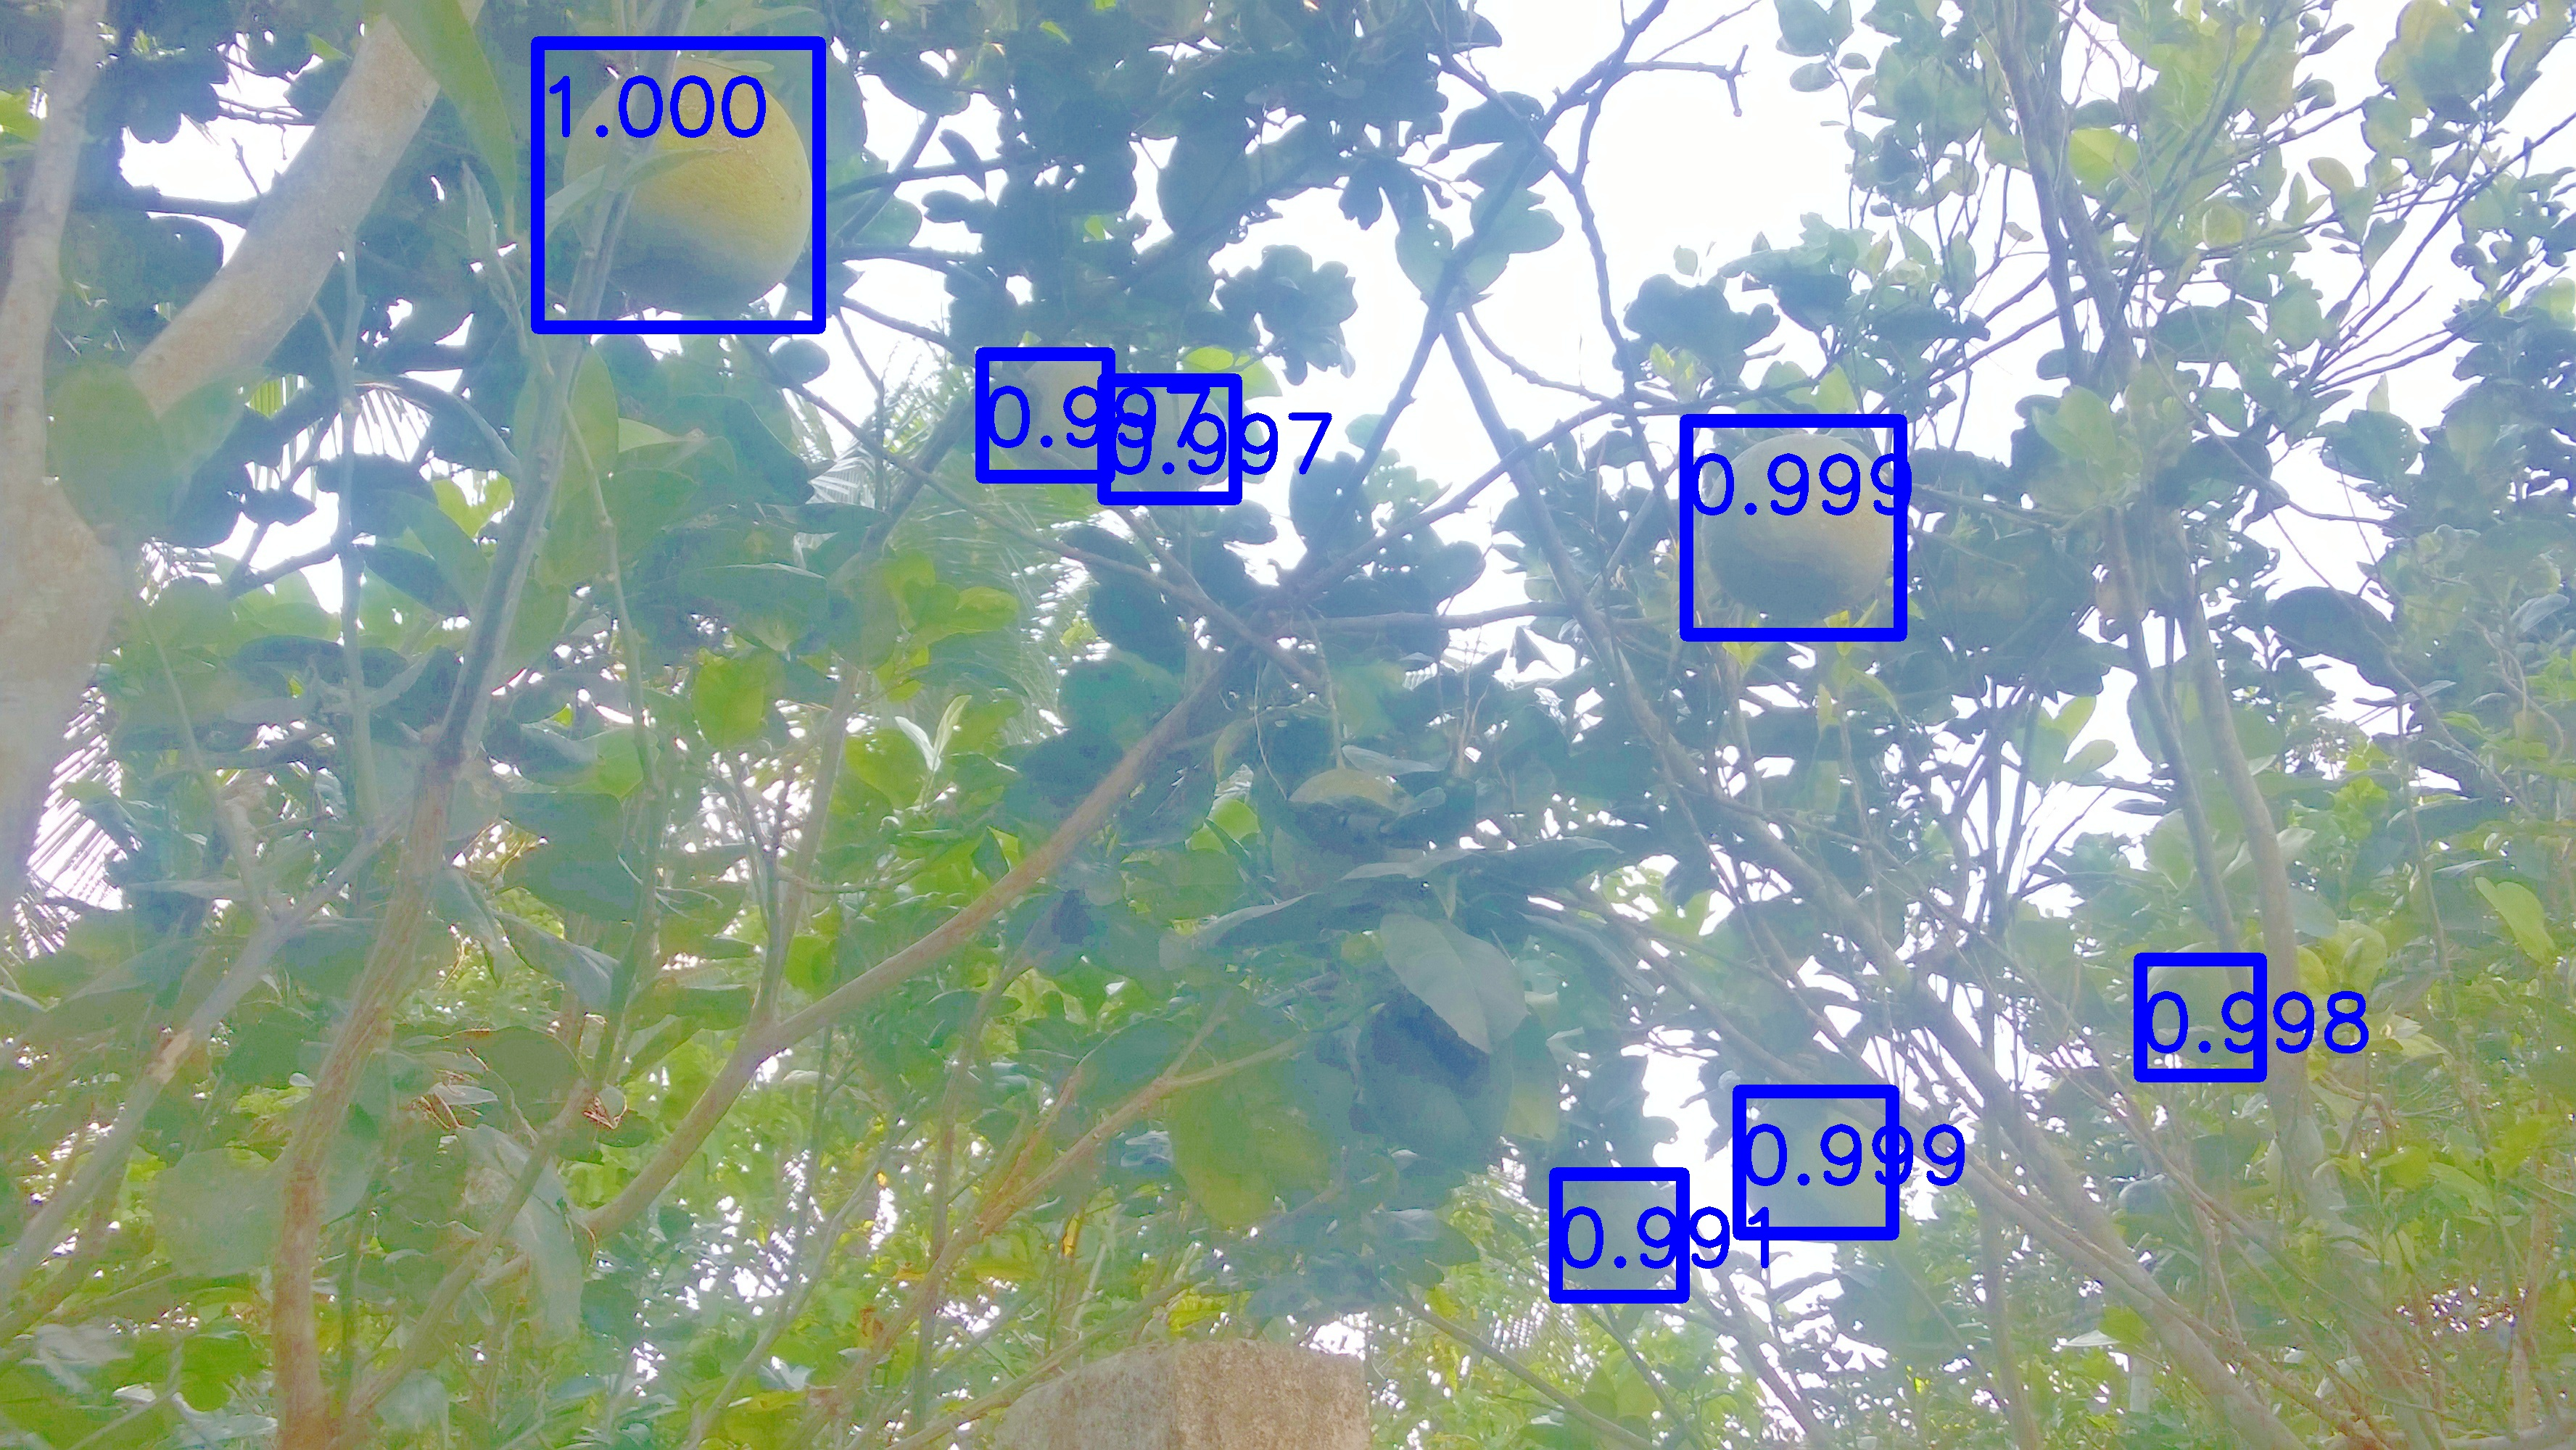
\includegraphics[width=0.6\columnwidth]{images/chap3/demo_012.jpg}
    \caption{Kết quả nhận diện với hình ảnh bị thay đổi độ sáng}
    \label{chap3:good6}
    \end{figure}
\end{center}

Hình \ref{chap3:lack1}, \ref{chap3:lack2}, \ref{chap3:lack3}Đối với trường hợp trái nằm cạnh vùng có nhiều lá, kết quả nhận diện vẫn rất khả quan, tuy nhiên vẫn còn một số vị trí bị nhận diện nhầm.

\begin{center}
    \begin{figure}[H]
    \centering
    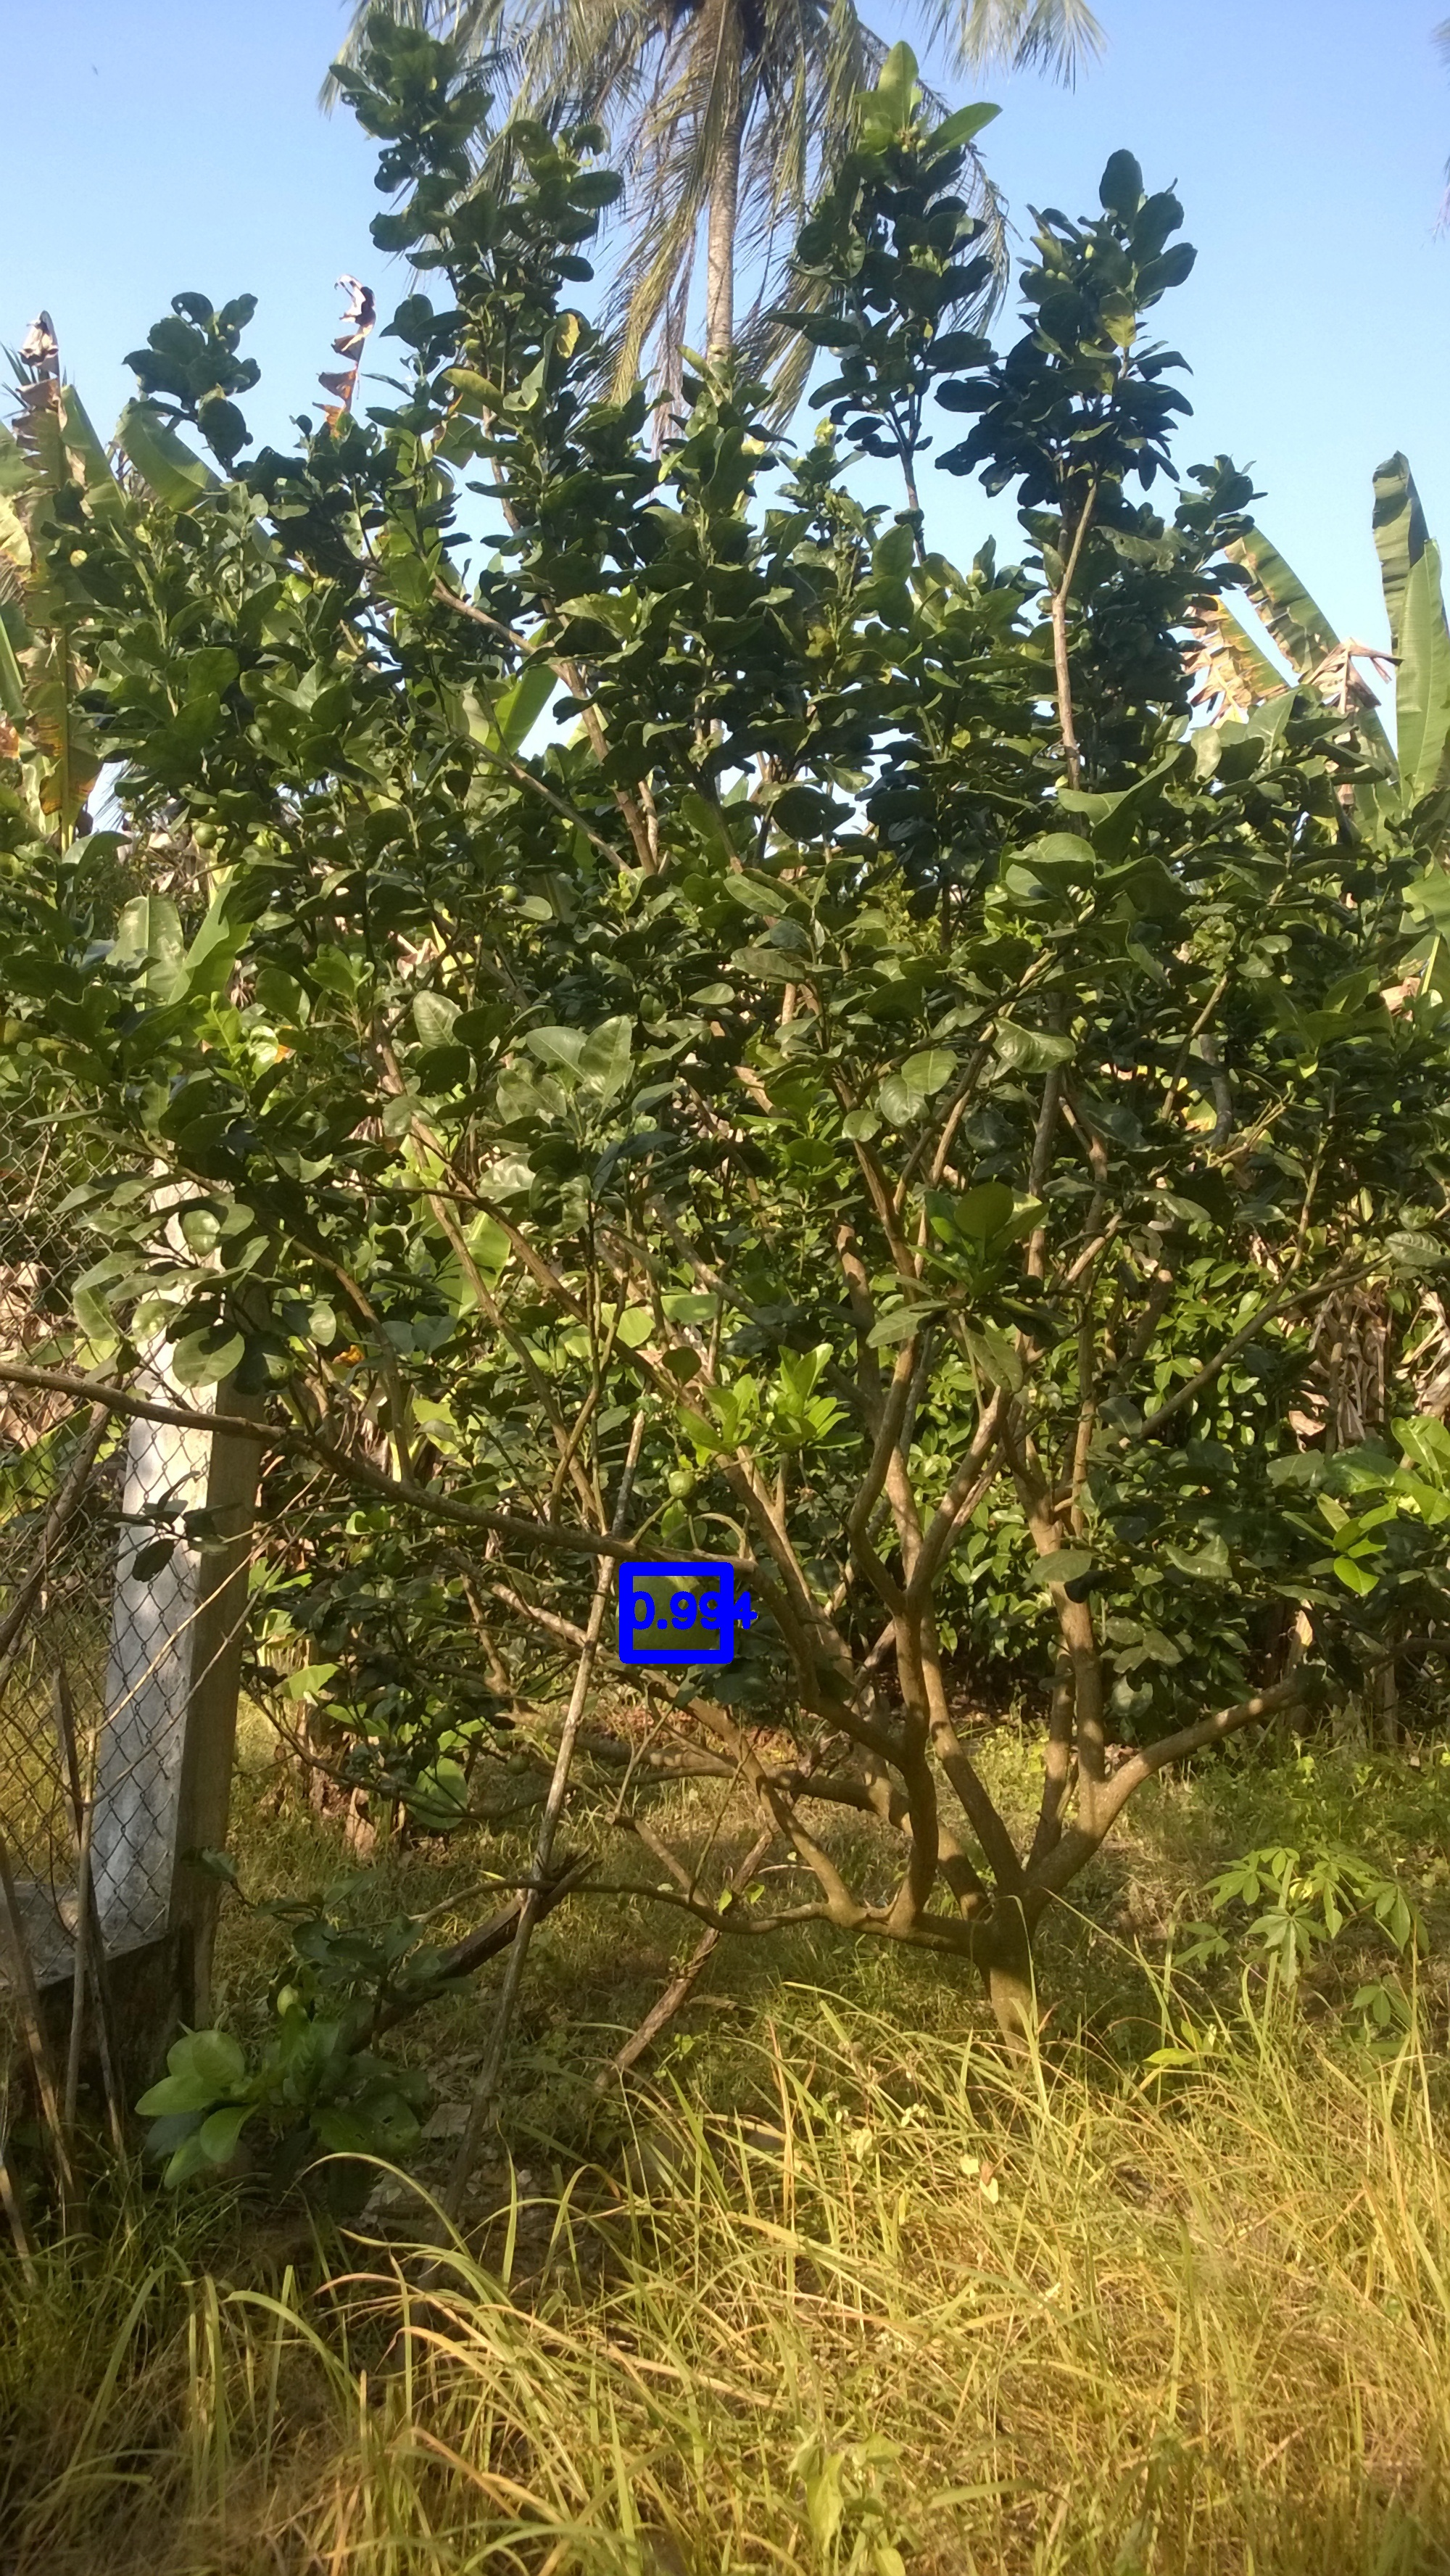
\includegraphics[width=0.7\columnwidth]{images/chap3/demo_008.jpg}
    \caption{Tuy nằm gần nhiều lá những trái bưởi vẫn được nhận diện tốt}
    \label{chap3:lack1}
    \end{figure}
\end{center}
\begin{center}
    \begin{figure}[H]
    \centering
    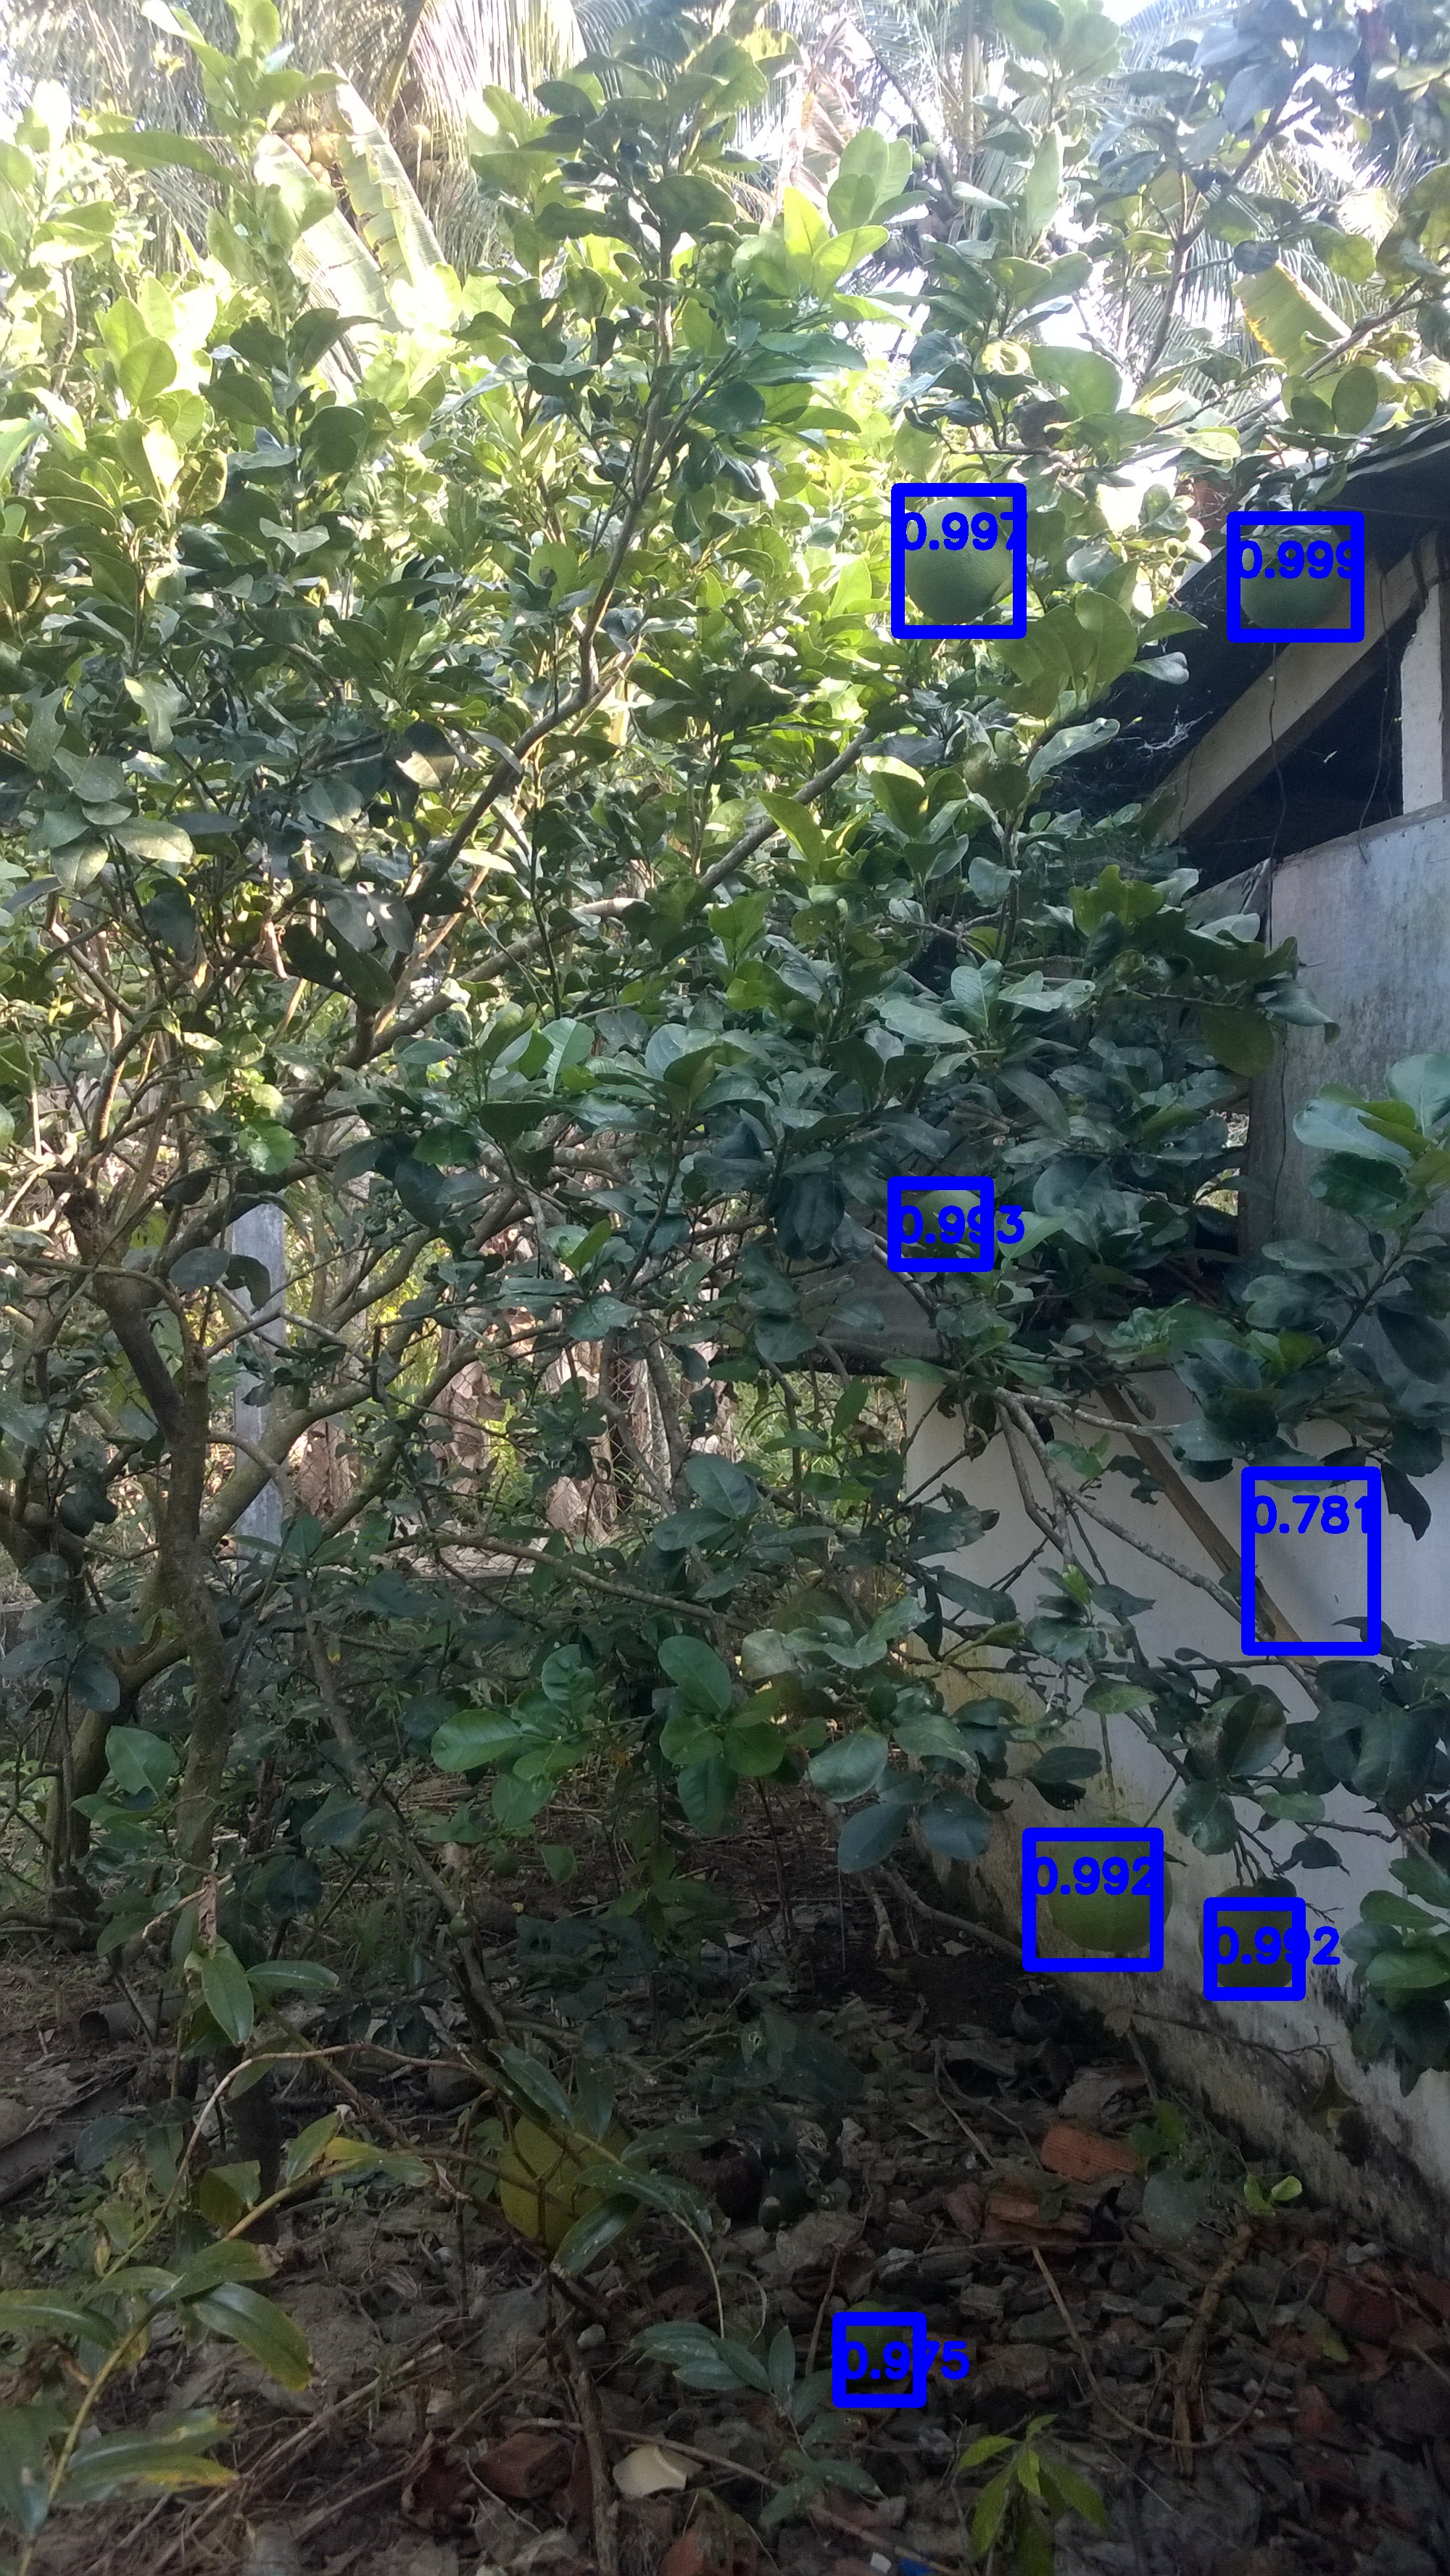
\includegraphics[width=0.7\columnwidth]{images/chap3/demo_009.jpg}
    \caption{Phần tường bị nhận diện nhầm thành bưởi}
    \label{chap3:lack2}
    \end{figure}
\end{center}
\begin{center}
    \begin{figure}[H]
    \centering
    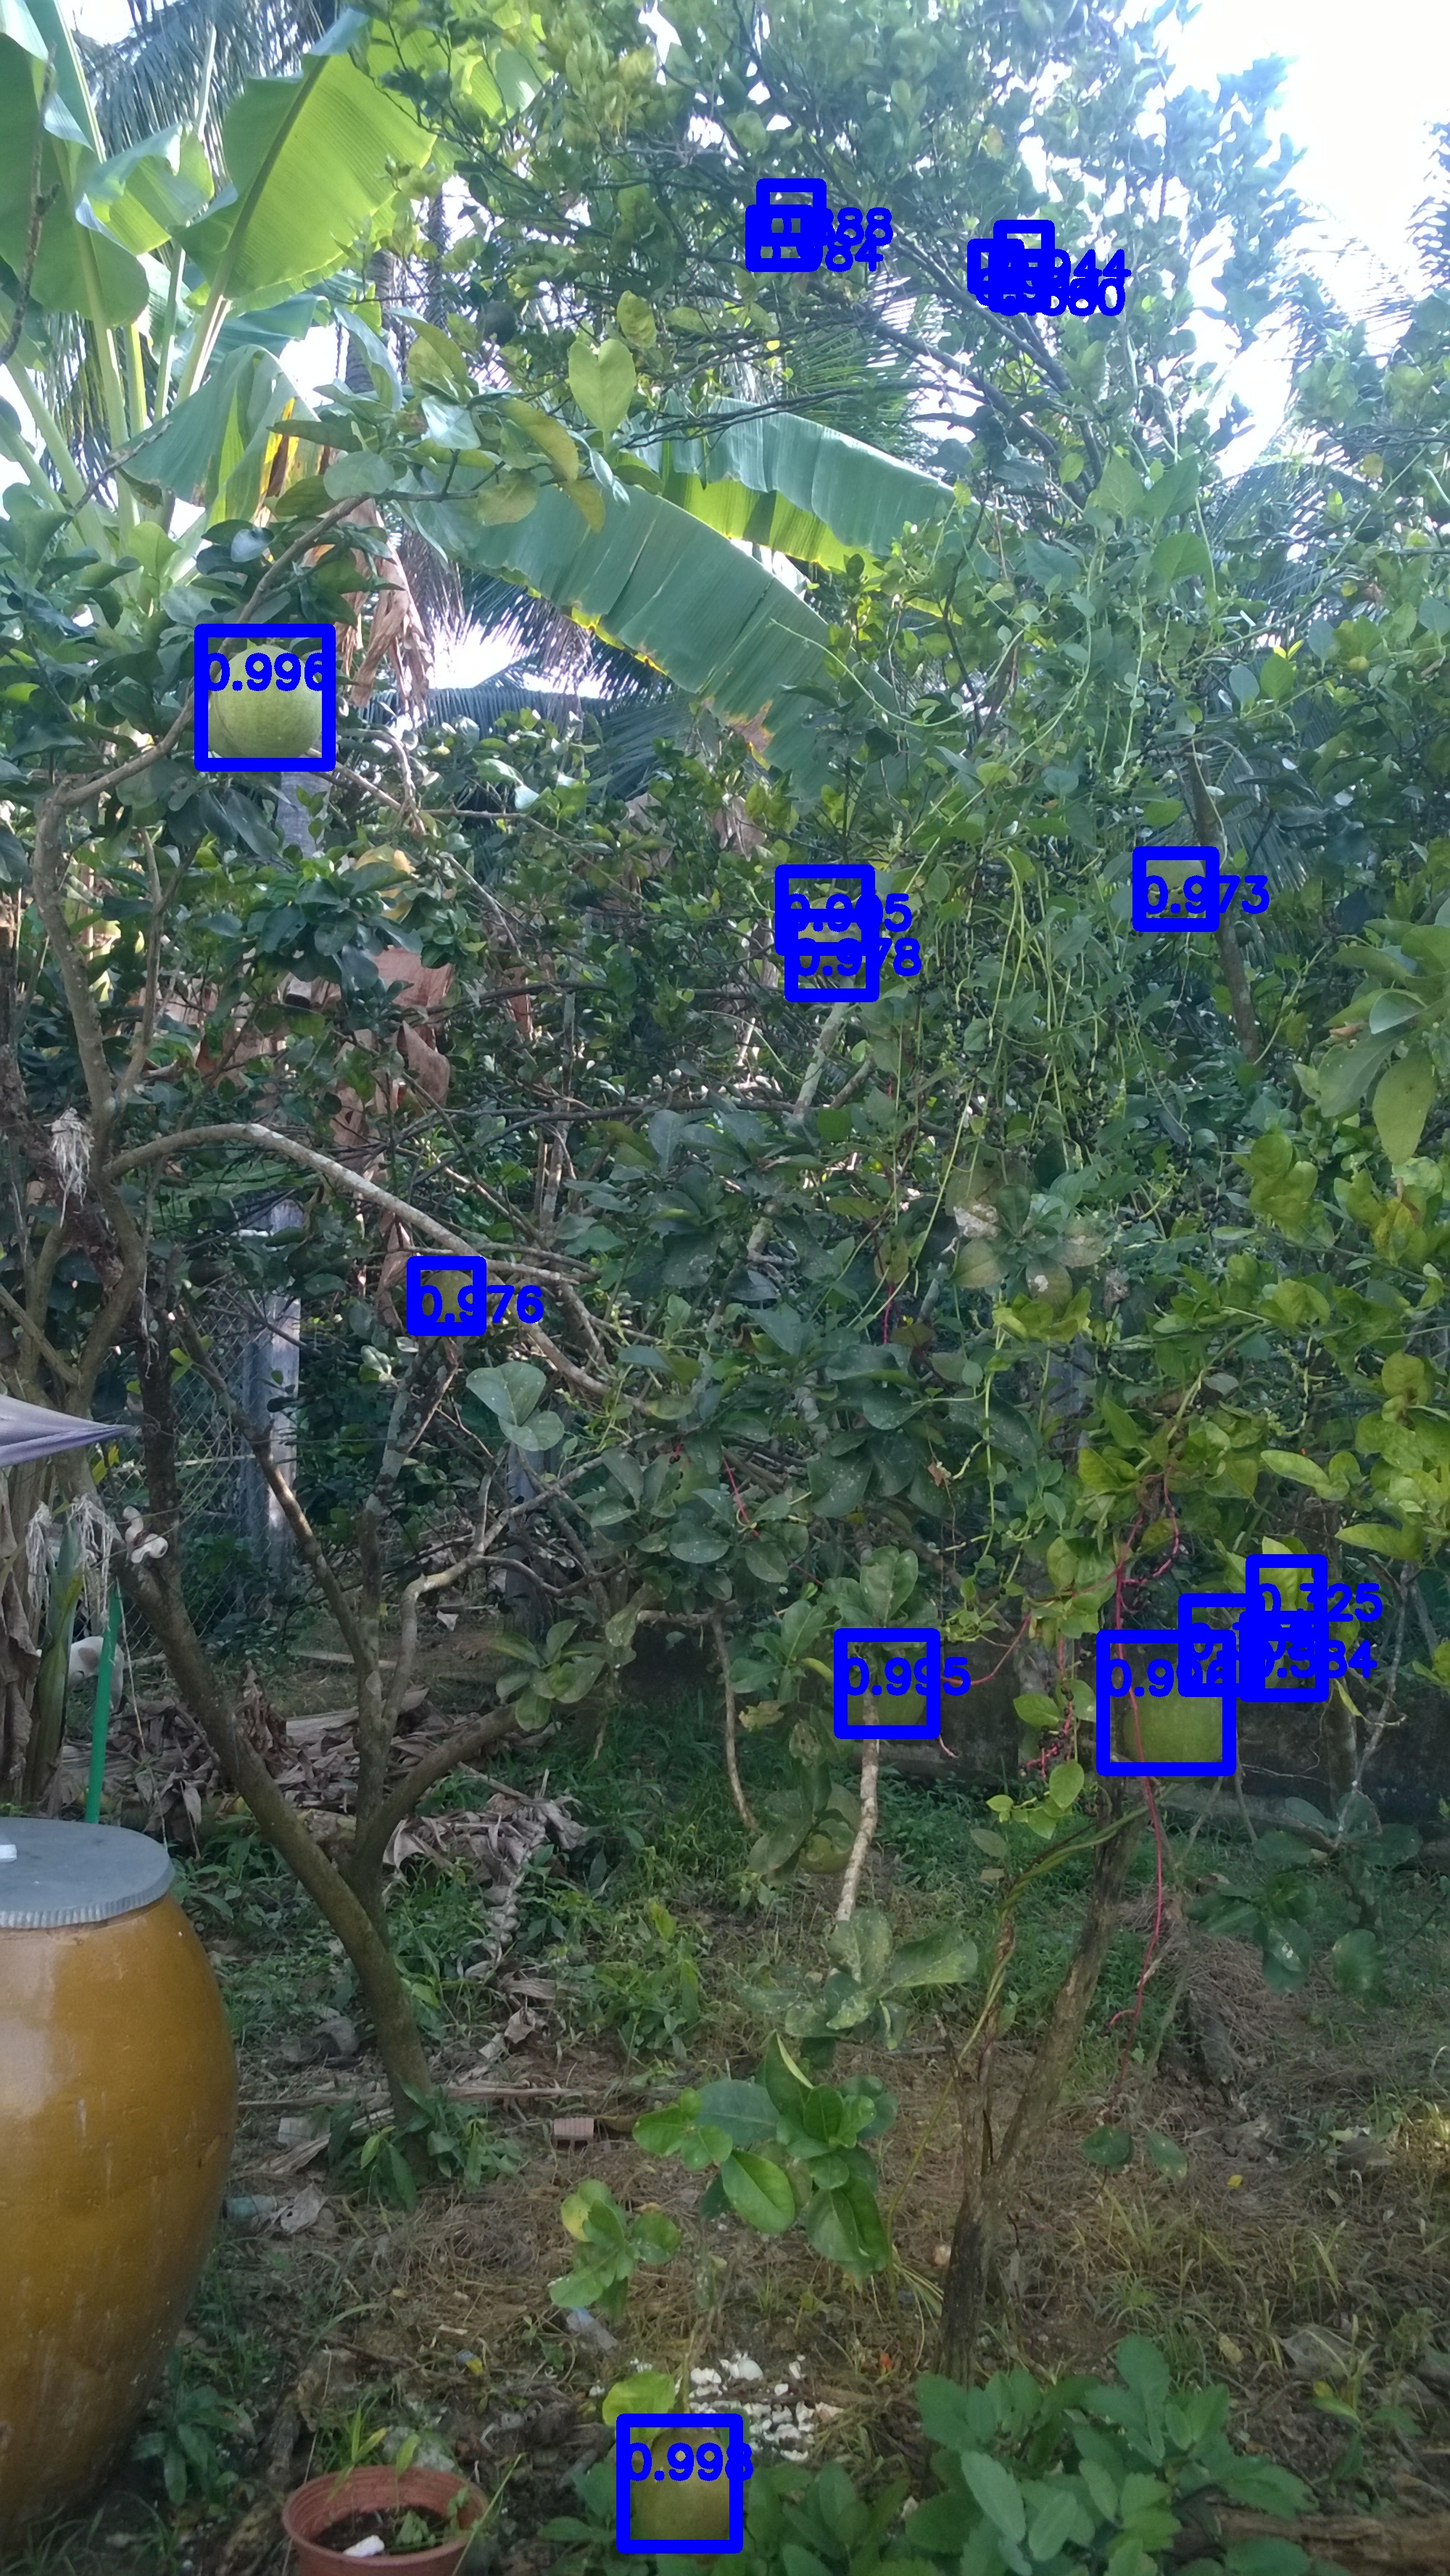
\includegraphics[width=0.7\columnwidth]{images/chap3/demo_010.jpg}
    \caption{Xuất hiện một ít vùng bị nhận diện trùng nhau khi trái bưởi quá nhỏ}
    \label{chap3:lack3}
    \end{figure}
\end{center}
